\documentclass[10pt,journal,compsoc]{IEEEtran}

\usepackage{cite}
\usepackage{graphicx}
\usepackage{amsmath}
\usepackage{amssymb}
\usepackage{amsthm}
\newtheorem{proposition}{Proposition}
\newtheorem{corollary}{Corollary}
\usepackage{array}
\usepackage{url}
\usepackage{color}
\usepackage{booktabs}
\usepackage{float}
\usepackage{subfig}
\usepackage{textcomp}
\usepackage{multirow}
\usepackage{overpic}
\usepackage{amsfonts}
\usepackage{xcolor,colortbl}
\usepackage{algorithmic}
\usepackage{algorithm}
\usepackage{enumitem}
\usepackage{placeins}

\definecolor{Gray}{gray}{.90}

\newcommand{\tabincell}[2]{\begin{tabular}{@{}#1@{}}#2\end{tabular}}
\newcommand{\etal}{\textit{et al}.}
\newcommand{\ie}{\textit{i}.\textit{e}.}
\newcommand{\eg}{\textit{e}.\textit{g}.}
\newcommand{\etc}{\textit{etc}.}

% subfigure label format handled by subfig package

\ifCLASSINFOpdf
\else
\fi

\usepackage[bookmarks,colorlinks,linkcolor=black, anchorcolor=black, citecolor=black, urlcolor=black]{hyperref}
\hyphenation{op-tical net-works semi-conduc-tor}


\begin{document}

\title{EDG++: Reliability-Aware Electron Density-Enhanced Molecular Geometry Learning}

\author{Hongxin Xiang, Siyu Wang, Zhixiang Cheng, Jun Xia, Xin Jin, Wenjie Du, Li Zeng, Hongbo Yang, and Xiangxiang Zeng,~\IEEEmembership{IEEE Senior Member}
\IEEEcompsocitemizethanks{\IEEEcompsocthanksitem \textit{(Hongxin Xiang and Siyu Wang are co-first authors.) (Corresponding authors: Hongbo Yang; Xiangxiang Zeng.)}
\IEEEcompsocthanksitem H. Xiang is with the College of Computer Science and Electronic Engineering, Hunan University, Changsha, China.
\IEEEcompsocthanksitem S. Wang is with the School of Life Sciences, East China Normal University, Shanghai, China.
\IEEEcompsocthanksitem Z. Cheng is with the College of Computer Science and Electronic Engineering, Hunan University, Changsha, China.
\IEEEcompsocthanksitem J. Xia is with the School of Engineering, Westlake University, Hangzhou, China.
\IEEEcompsocthanksitem X. Jin is with the Eastern Institute of Technology, Ningbo, China.
\IEEEcompsocthanksitem W. Du is with the University of Science and Technology of China, Hefei, China.
\IEEEcompsocthanksitem L. Zeng is with the College of Computer Science and Electronic Engineering, Hunan University, Changsha, China.
\IEEEcompsocthanksitem H. Yang is with the Institute of Reproduction and Development, Fudan University, Shanghai, China (e-mail: hongboyang@fudan.edu.cn).
\IEEEcompsocthanksitem X. Zeng is with the College of Computer Science and Electronic Engineering, Hunan University, Changsha, China (e-mail: xzeng@hnu.edu.cn).
}
}

\markboth{IEEE Transactions on Pattern Analysis and Machine Intelligence}%
{Xiang \MakeLowercase{\textit{et al.}}: EDG++: Reliability-Aware Electron Density-Enhanced Molecular Geometry Learning}

\IEEEtitleabstractindextext{
\begin{abstract}
% [Polish] Original: Electron density (ED) encodes the electronic-structure information that drives quantum molecular properties, yet computing it for every prediction is prohibitively expensive. We propose EDG, a cross-modal distillation framework that transfers ED knowledge from a pre-trained ED-aware teacher to geometry students as privileged information, requiring no ED computation at inference. Naive distillation, however, treats every teacher prediction as equally trustworthy and risks negative transfer; we therefore extend EDG to EDG++, which gates supervision through a pre-trained reliability estimator with adaptive thresholding, and prove (Proposition~1) a sufficient condition under which gating reduces an upper bound on gradient noise---yielding gains on 34/36 QM9 tasks, 55/60 rMD17 energy/force tasks, and 27--38\% tail-error reduction on the hardest 1\% of samples. As a stress test on the 166-atom mini-protein Chignolin---substantially out of the teacher's training distribution---naive EDG measurably degrades the baseline ($+\!4.0\%$ energy, $+\!2.8\%$ force MAE) while EDG++'s gating recovers a net improvement ($-\!6.8\%$ energy, $-\!2.9\%$ force), and the same frozen estimator additionally serves as an inference-time OOD detector during MD rollouts.
Electron density (ED), which describes the spatial distribution of electrons in a molecule, is crucial for accurately predicting the energies and forces in molecular force fields (MFF). However, existing MLFF methods exploit only atom-level geometric quantities and ignore the electronic-level information that governs these properties. To bridge this gap, we propose EDG, a cross-modal knowledge distillation framework that transfers ED knowledge from a pre-trained ED-aware teacher to geometry-based students at training time; at inference, only the geometry student is used, avoiding the prohibitive cost of quantum chemical calculations. Since naive distillation treats every teacher prediction as equally trustworthy and can lead to negative transfer, we further propose EDG++, which gates the distillation signal through a pre-trained reliability estimator with adaptive thresholding; a theoretical analysis shows that the gating reduces an upper bound on the gradient noise. Extensive experiments on QM9 and rMD17 show that the framework can be directly integrated into a wide range of geometry-based models (SchNet, Equiformer, SphereNet, ViSNet), significantly improving their geometric representation learning capability with a maximum average improvement of 33.7\%, with consistent gains on 34/36 QM9 task-model combinations and 55/60 rMD17 energy/force tasks. On the 166-atom mini-protein Chignolin, far outside the teacher's training distribution, EDG++ further demonstrates the rescue effect of reliability gating against the negative transfer induced by naive distillation. EDG/EDG++ offers a general framework for injecting electronic-level inductive bias into geometric molecular models, with applications to molecular property prediction, ML force field learning, and biomolecular dynamics simulation.
\end{abstract}

\begin{IEEEkeywords}
Electron density, molecular geometry learning, knowledge distillation, reliability-aware learning, machine learning force fields.
\end{IEEEkeywords}

}

\maketitle

\IEEEdisplaynontitleabstractindextext
\IEEEpeerreviewmaketitle

\section{Introduction}
\label{sec:Introduction}

Machine learning force fields (MLFF) provide a computationally efficient and low-cost approach to learning the interactions between atoms, bringing revolutionary advances to molecular dynamics simulations across physics, chemistry, biology, and materials science~\cite{behler2007generalized,unke2021machine,chmiela2017machine,xiang2024molecular,wang2024efficiently}. However, current MLFF methods, built on geometric deep learning with E(3)-equivariant architectures~\cite{thomas2018tensor,fuchs2020se3,liu2022spherical,wang2024enhancing}, focus on atom-level physical quantities such as coordinates and multi-body interactions~\cite{batzner20223,liao2023equiformer,wang2024enhancing}, while ignoring information at the electronic level.

Electron density (ED) describes the probability density of finding an electron at a given point in three-dimensional space and is a foundational quantity for predicting the quantum chemical properties of MFF~\cite{sunshine2023chemical,skogh2024electron}. The Hohenberg-Kohn theorem~\cite{hohenberg1964inhomogeneous} formalizes this relationship by establishing that the ground-state energy is a unique functional of the electron density. Despite this central role, exploiting ED in MLFF faces three major challenges:

\begin{figure*}[htbp]
\centering
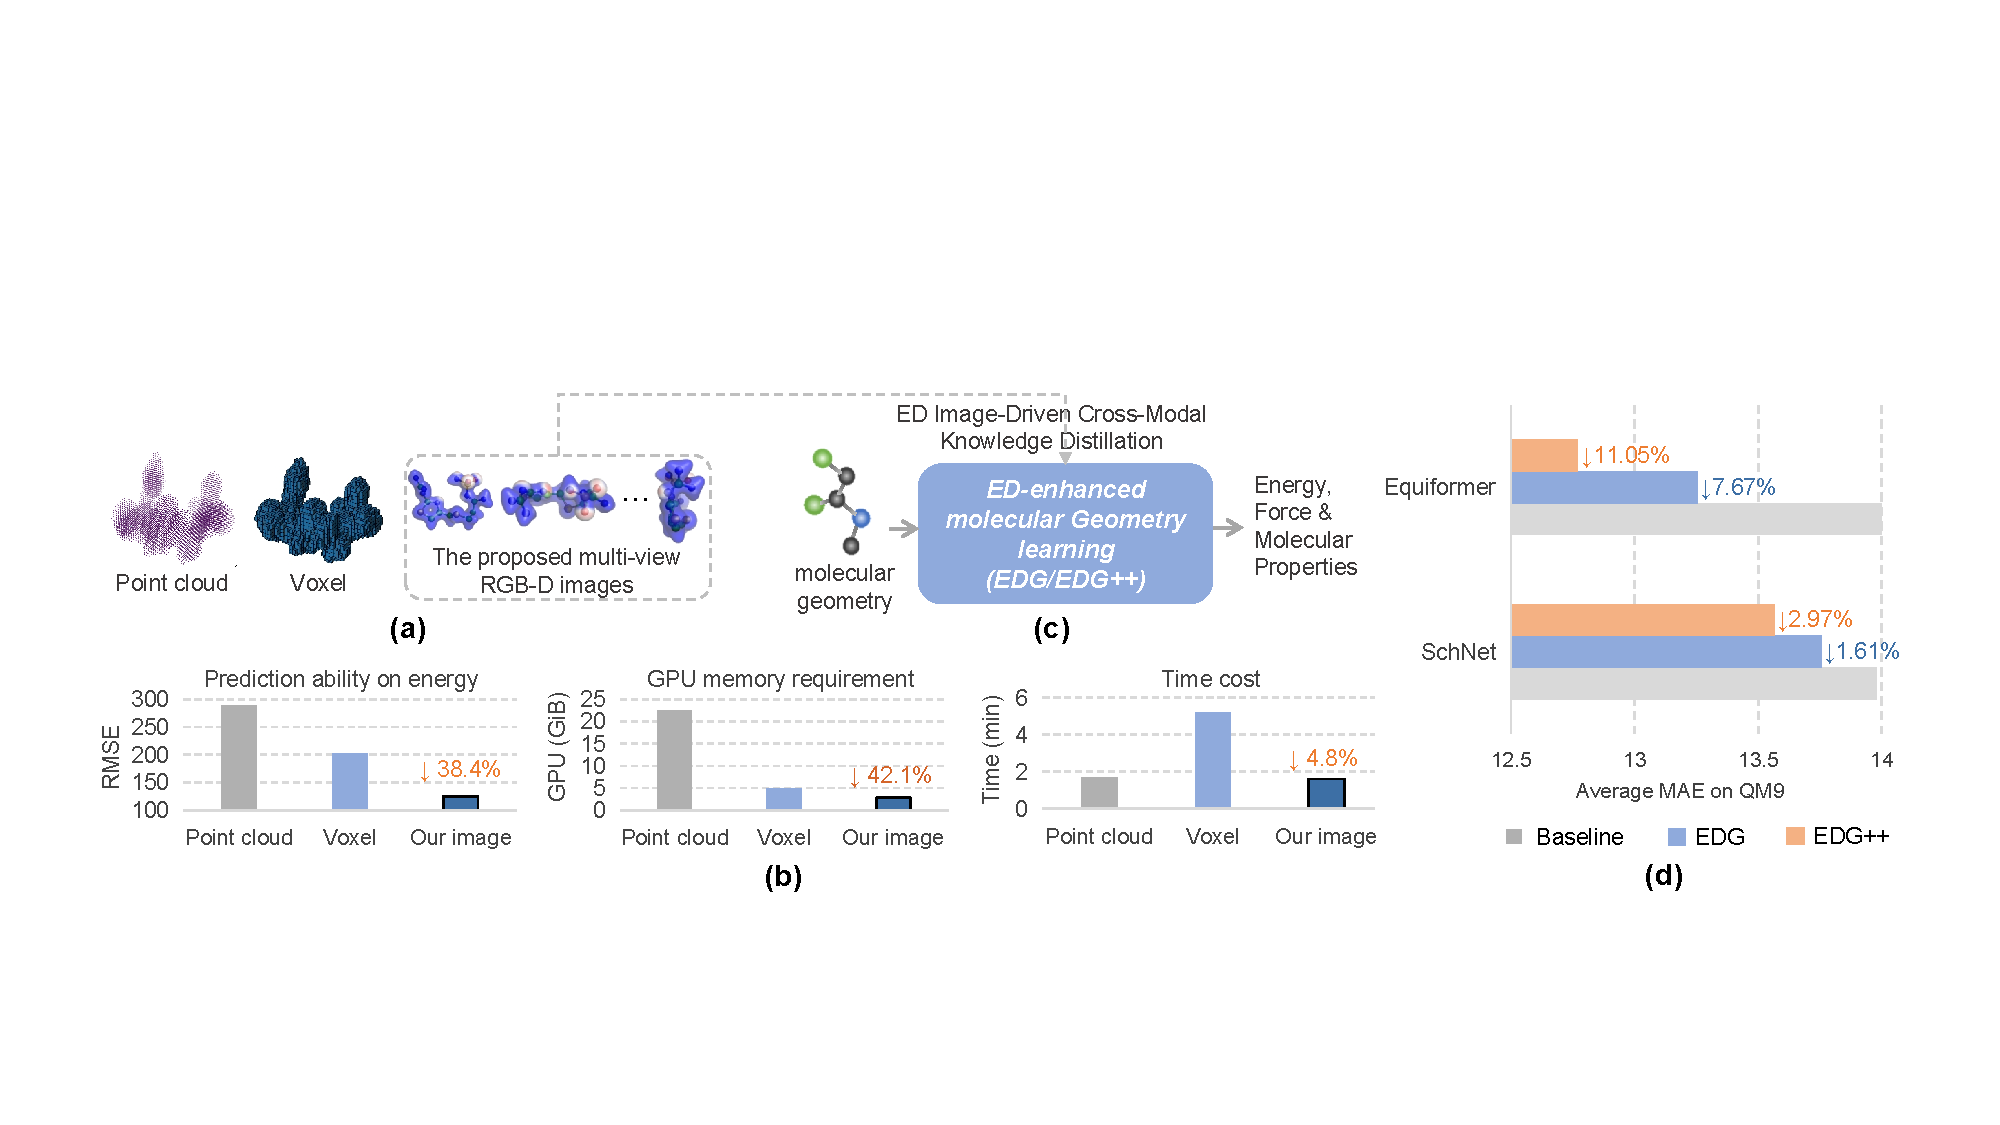
\includegraphics[width=\textwidth]{imgs_edgpp/introduction/fig1_introduction.pdf}
\caption{Motivation and overview (detailed pipeline in Fig.~\ref{Fig2_Method}). (a) ED representation methods. (b) RMSE, GPU memory, and training time of different ED representations. (c) High-level EDG/EDG++ framework: multi-view ED images with RGB-D channels enhance molecular geometry learning; EDG++ adds reliability-aware selective distillation. (d) Average MAE on 12 QM9 tasks. EDG improves both SchNet and Equiformer; EDG++ further improves through reliability-aware selective distillation.}
\label{Fig1_Intro}
\end{figure*}

% [Polish] Original: \textit{Challenge 1: High computational complexity of ED.} Unlike the number of atoms in a molecule, which is usually on the scale of tens to hundreds, the ED relies on a continuous spatial distribution and as the resolution increases, the number of data points may reach millions or even tens of millions. As shown in Fig.~\ref{Fig1_Intro}(a), there are two direct ways to represent ED: point cloud~\cite{guo2020deep} and voxel~\cite{gong2023incorporation}. As shown in Fig.~\ref{Fig1_Intro}(b), we empirically show the limitations of point clouds and voxels as ED representations in energy prediction, GPU memory efficiency, and training efficiency. In particular, point clouds and voxels are directly related to the resolution of the ED, so the computational efficiency will decrease as the resolution increases. These limitations motivate us to propose a multi-view RGB-D image (the right subfigure of Fig.~\ref{Fig1_Intro}(a)) for accurate and efficient ED representation, which produces a fixed-size output regardless of ED grid resolution and compresses the continuous ED signal into pixels. Compared with point clouds and voxels, the proposed images improve energy prediction ability, GPU memory efficiency, and training efficiency by 38.4\%, 42.1\%, and 4.8\%, respectively.
\textit{Challenge 1: High computational complexity of ED.} ED is defined on a continuous spatial domain, with grid points reaching millions or tens of millions as resolution increases---far larger than the tens-to-hundreds scale of atomic nodes. As shown in Fig.~\ref{Fig1_Intro}(a), existing approaches represent ED as either point clouds~\cite{guo2020deep} or voxels~\cite{gong2023incorporation}, both suffering from two limitations: (1)~limited energy-prediction accuracy due to information loss in discretization (Fig.~\ref{Fig1_Intro}(b)); (2)~GPU memory and training cost that scale directly with ED resolution. To address both limitations, we propose a multi-view RGB-D image representation (right subfigure of Fig.~\ref{Fig1_Intro}(a)) that produces a fixed-size output independent of ED grid resolution and compresses the continuous ED signal into pixels. Compared with point clouds and voxels, our representation improves energy prediction, GPU memory efficiency, and training efficiency by 38.4\%, 42.1\%, and 4.8\%, respectively.

\textit{Challenge 2: Expensive ED acquisition.} Obtaining ground-state ED at the level required by MFF relies on computationally intensive quantum chemical calculations such as density functional theory (DFT)~\cite{kohn1965self,hegde2017machine,lee2024convolutional}, which demand substantial computing resources and become prohibitive at scale. As shown in Fig.~\ref{Fig1_Intro}(c), we recast ED-enhanced geometry learning as a teacher-student paradigm: we first use DFT to compute 2 million high-quality ED examples and pre-train an ED representation learning model (ImageED); we then transfer this knowledge to an ED-aware teacher that takes ED-free structural images as input, which subsequently distills geometry students. This scheme, called \textbf{EDG} (Electron Density-enhanced Geometry learning), requires ED computation only once during pre-training and eliminates the need for ED data in all downstream stages. As shown in Fig.~\ref{Fig1_Intro}(d), geometry students equipped with EDG achieve consistent improvements on QM9. However, this naive scheme treats all teacher predictions equally, which motivates the third challenge below.

\textit{Challenge 3: Unreliable teacher predictions causing negative transfer.} Beyond feasibility and efficiency, a critical question remains: \emph{when should we trust the teacher's predictions?} The quality of cross-modal predictions varies across samples due to intrinsic DFT approximations, molecular conformation diversity, and information loss when compressing 3D electron clouds into 2D images. \emph{Naive distillation implicitly assumes uniform teacher fidelity, risking negative transfer}~\cite{pan2010survey}. To address this, we propose \textbf{EDG++}, a reliability-aware extension that introduces a pre-trained reliability estimator and an adaptive global-local thresholding mechanism for selective distillation, filtering unreliable teacher predictions before knowledge transfer (Section~\ref{sec:Theoretical_Analysis}--\ref{sec:Adaptive_Thresholding}). Equipped with this mechanism, EDG++ achieves consistent improvements on 34/36 QM9 task-model combinations and 55/60 rMD17 energy/force tasks, with up to 27--38\% tail-error reduction on the hardest 1\% of samples.

We summarize the main contributions as follows:
\begin{itemize}[itemsep=2pt,topsep=0pt,parsep=0pt]
    \item We propose multi-view RGB-D images as an efficient and resolution-independent representation of electron density, and develop ImageED, a masked autoencoder that learns ED-related features from this representation.
    \item Building on ImageED, we propose EDG, a cross-modal distillation framework that transfers ED knowledge to geometry-based MLFF models through an ED-aware teacher, with no additional computational cost at inference.
    \item We further propose EDG++, integrating a pre-trained reliability estimator with an adaptive global-local thresholding mechanism for selective distillation to mitigate negative transfer.
    \item Extensive experiments validate EDG/EDG++ across diverse student architectures: SchNet, Equiformer, and SphereNet on QM9; SchNet, SphereNet, and ViSNet on rMD17. EDG++ improves on 34/36 QM9 task-model combinations and 55/60 rMD17 energy/force tasks.
    \item We design an out-of-distribution case study on the 166-atom mini-protein Chignolin (Sec.~\ref{sec:case_study_chignolin}), where EDG++'s reliability gating successfully mitigates negative transfer in realistic OOD settings.
\end{itemize}

\textbf{Difference with Conference Version.} Table~\ref{tab:conf_vs_journal} summarizes the key differences between the IJCAI 2025 conference paper~\cite{xiang2025edg} (EDG) and this journal extension (EDG++).

\begin{table}[!htb]
  \centering
  \caption{Conference (IJCAI 2025) vs.\ journal extension.}
  \label{tab:conf_vs_journal}
  \scriptsize
  \setlength{\tabcolsep}{3pt}
  \begin{tabular}{@{}lcc@{}}
    \toprule
    \textbf{Aspect} & \textbf{Conference (EDG)} & \textbf{Journal (EDG++)} \\
    \midrule
    Distillation & Naive (all samples) & Selective (reliability-aware) \\
    Reliability est.\ & -- & Pre-trained; \texttildelow131K params \\
    Thresholding & -- & Adaptive global-local \\
    Architecture cov.\ & EDG only & EDG++ on all three \\
                       &          & students per benchmark \\
    Ablations & $\lambda$ only & $\beta$ (hybrid), $\kappa$ (strictness) \\
    OOD case study & -- & Chignolin (166 atoms) \\
    \bottomrule
  \end{tabular}
\end{table}

\section{Related Work}
\label{sec:RelatedWork}

\subsection{Molecular Geometry Representation Learning}

Geometric deep learning drives the progress of machine learning force fields (MLFF)~\cite{liu2022spherical,wang2024enhancing}. Equivariant neural networks (ENNs)~\cite{satorras2021n} that respect E(3) symmetries are the dominant paradigm, with methods modeling inter-atomic interactions~\cite{schutt2017schnet,liao2023equiformer}, angular information~\cite{gasteiger2020directional,liu2022spherical,gasteiger2021gemnet}, and higher-order representations~\cite{liao2024equiformerv2,passaro2023reducing,wang2024enhancing}. However, all existing geometry-based methods operate solely on nuclear-level information and do not incorporate electronic structure. Our approach is architecture-agnostic and supplements any geometric model with electronic information.

\subsection{Electron Density Representation Learning}

Existing electron density (ED) representations fall into two categories. Point cloud methods treat all density values as a point set; for example, PointNet~\cite{qi2017pointnet} has been applied to classify the symmetry of inorganic compounds~\cite{kim2024deep}. Voxel methods discretize the density field on a regular grid; 3D CNNs~\cite{liu2015sparse} have been used to predict molecular exchange energy~\cite{gong2023incorporation} and discover host-molecule guests~\cite{parrilla2024electron}, while 3D-UNet~\cite{cciccek20163d} segments reactive sites and classifies substances~\cite{singh2024classification}.

Beyond direct ED representation, several works have explored machine learning approaches to predict or bypass electron density computation. Brockherde~\etal~\cite{brockherde2017bypassing} proposed bypassing the Kohn-Sham equations by directly learning the density-to-energy mapping. Nagai~\etal~\cite{nagai2020completing} used neural networks to learn the exchange-correlation functional from molecular electron densities. Sunshine~\etal~\cite{sunshine2023chemical} predicted chemical properties from GNN-predicted electron densities, demonstrating that learned ED representations carry meaningful chemical information. More recently, Lee~\etal~\cite{lee2025selfsupervised} proposed self-supervised diffusion processes for electron-aware molecular representation learning, and Gao~\etal~\cite{gao2025equivariant} developed equivariant non-local electron density functionals. However, these methods either require ED at inference time, focus on predicting ED itself, or learn ED-aware representations without a cross-modal distillation mechanism. % [Polish] Original: Different from previous methods, we propose a novel multi-view RGB-D image to represent ED and design a representation learning method to extract features, enabling ED knowledge to be transferred to geometry models without requiring ED at inference.
In contrast, we represent ED as multi-view RGB-D images and design a representation learning method to extract features, enabling ED knowledge to be transferred to geometry models without requiring ED at inference.

\subsection{Knowledge Distillation and Privileged Information}

Knowledge distillation (KD)~\cite{hinton2015distilling,gou2021knowledge} transfers knowledge from a teacher model to a student model, typically by matching soft predictions or intermediate representations. Feature-based distillation methods~\cite{romero2015fitnets,zagoruyko2017paying} extend this paradigm by aligning intermediate layer activations. Wang~\etal~\cite{wang2021knowledge} provided a comprehensive review. Recent work has recognized that not all teacher knowledge is equally beneficial. In the selective KD line, SelKD~\cite{park2024selkd} formulates selection via optimal transport, and Shi~\etal~\cite{shi2025selkd} further develop this perspective at scale. Studies on teacher calibration~\cite{guo2017calibration,das2023understanding} and uncertainty-aware teaching~\cite{lin2023teaching,guo2023selective} have shown that accounting for the teacher's confidence can significantly improve outcomes.

Cross-modal KD is increasingly studied~\cite{huo2024c2kd}, showing that bridging heterogeneous feature spaces requires explicit alignment. Our framework distills between fundamentally different representations---ED images and atomic graphs---where the representational and symmetry gap poses distinct challenges.

\textbf{Positioning of EDG++.} We distinguish four sources of unreliable supervision: (1) \emph{sample difficulty}~\cite{bengio2009curriculum,kumar2010self}; (2) \emph{label noise}~\cite{han2018co,song2022learning}; (3) \emph{teacher uncertainty}~\cite{park2024selkd,shi2025selkd}; (4) \emph{cross-modal alignment quality}---where the cross-modal mapping itself is imperfect for certain samples. EDG++ operates in category (4): task labels are clean, but the quality of the cross-modal prediction varies due to information loss in the 3D-to-2D projection. This motivates a reliability estimator that predicts the teacher's reconstruction error, rather than relying on the teacher's own uncertainty. Our work builds upon the LUPI paradigm~\cite{vapnik2009new,lopez2016unifying}, with electron density as the privileged modality. Additional discussion of selective learning methods is provided in Appendix~\ref{sec:appendix_selective_learning}.

\section{Our Method}
\label{sec:OurMethod}

\subsection{Preliminaries}

\textbf{Privileged information setup.} Following the LUPI paradigm~\cite{vapnik2009new,lopez2016unifying}, we treat ED as \emph{privileged information}: it is computed via DFT during training but is not required at inference, eliminating the cost of quantum chemical computation at deployment.

\textbf{Notation and Problem Formulation.} The molecular geometry and the corresponding ground-truth labels with $k$ prediction tasks are $\{\mathcal{G}_i=(\mathcal{V}_i, \mathcal{E}_i)\}_{i=1}^n$ and $\{y_i\}_{i=1}^n\in\mathbb{R}^k$ respectively, where $\mathcal{V}_i\in\mathbb{R}^{n^v_i\times(3+d_i^v)}$ ($n^v_i$, 3, $d_i^v$ are the number of atoms, the coordinates, and the feature dimensions) and $\mathcal{E}_i\in\mathbb{R}^{n^e_i\times d_i^e}$ ($n^e_i$ is the number of edges and $d_i^e$ is the feature dimensions of bonds). The corresponding multi-view ED image and structural image are $\mathcal{U}\in\mathbb{R}^{N_v\times 4\times H\times W}$ and $\mathcal{S}\in\mathbb{R}^{N_s\times 3\times H\times W}$ respectively, where $N_v$ and $N_s$ denote the number of views for ED images ($N_v\!=\!6$) and structural images ($N_s\!=\!4$), and $H$, $W$ are the image height and width. 3 and 4 represent RGB and RGB-D channels, respectively.

The framework comprises three stages: (1) pre-train a masked autoencoder (MAE)~\cite{he2022masked} with ED encoder $f_{EDE}$ and decoder $f_{EDD}$ to learn representations $\mathcal{F}^{\mathcal{U}}\in\mathbb{R}^{d^U}$ from ED images $\mathcal{U}$; (2) jointly pre-train an ED-aware teacher $f_{S}$, ED predictor $f_{EDP}$, and reliability estimator $\phi_{eval}$ to map structural images $\mathcal{S}$ to structural features $\mathcal{F}^{\mathcal{S}}\in\mathbb{R}^{d^{S}}$, then to ED-related features $\mathcal{F}^{\mathcal{S}\rightarrow\mathcal{U}}\in\mathbb{R}^{d^U}$, and to predict the teacher's per-sample reconstruction error; (3) distill a geometry student $f_{G}$ using the ED-aware teacher, ED predictor, reliability estimator, and mapper $f_M$ with selective distillation.

\subsection{Overview of the Method}

We propose \textbf{EDG} (\textbf{E}lectron \textbf{D}ensity-enhanced \textbf{G}eometry learning) and its reliability-aware extension \textbf{EDG++}. As shown in Fig.~\ref{Fig2_Method}, the framework has four modules: (a) 2 million molecular conformations are processed with DFT to produce multi-view ED images with RGB-D channels (Section~\ref{sec:Generation_ED_Image}); (b) ImageED learns ED-related representations from these images via two self-supervised tasks (Section~\ref{sec:ED_representation_learning}); (c) an ED-aware teacher is trained to predict ED features from structural images by minimizing the discrepancy with ImageED features (Section~\ref{sec:Pretraining_of_ED-aware_Teacher}); (d) the teacher distills ED knowledge into a geometry student through an ED predictor and mapper (Section~\ref{sec:ED-enhanced_Molecular_Geometry_Learning}). EDG++ extends the base framework with a theoretical analysis of when selective distillation reduces gradient noise (Section~\ref{sec:Theoretical_Analysis}), a reliability estimator (Section~\ref{sec:Reliability_Estimator}), and an adaptive thresholding mechanism (Section~\ref{sec:Adaptive_Thresholding}). Algorithm~\ref{alg:edg_process} in Appendix~\ref{sec:appendix_algorithm} summarizes the full three-stage pipeline.

\begin{figure*}[!htb]
\centering
\includegraphics[width=\textwidth]{imgs_edgpp/our_method/EDG++框架图_en.png}
\caption{Overview of the proposed EDG/EDG++ framework. \textbf{(a)} Multi-view ED images with RGB-D channels are generated based on 2 million molecular conformers and DFT data, which contains the structural and ED information of the molecule. \textbf{(b)} ImageED with masked autoencoder architecture and 2 pretext tasks ($\mathcal{L}_{VR}$ and $\mathcal{L}_{MR}$) is pretrained to extract ED-related features from multi-view ED images in (a). \textbf{(c)} The ED-aware teacher takes the structural images as input and learns to transform them into ED features $\mathcal{F}^{\mathcal{S}\rightarrow\mathcal{U}}$ using ED predictor and ED encoder in (b). The reliability estimator $\phi_{eval}$ is trained to predict the reconstruction error. \textbf{(d)} In downstream tasks, the ED-aware teacher, ED predictor, and reliability estimator from (c) are frozen to enhance the geometry student. EDG uses naive distillation while EDG++ uses reliability-aware selective distillation with adaptive thresholding. Electron density is no longer required at this stage, as the frozen ED-aware teacher already encodes ED-related information from structural images alone.}
\label{Fig2_Method}
\end{figure*}

\subsection{Generation of RGB-D Electron Density Images}
\label{sec:Generation_ED_Image}

We adopt the multi-view RGB-D rendering protocol of EDG~\cite{xiang2025edg}, summarized here for self-containment. As shown in Fig.~\ref{Fig2_Method}(a), 2 million conformations from PCQM4Mv2~\cite{hu2021ogb} are processed using DFT calculations~\cite{turney2012psi4} to obtain ED and electrostatic potential (ESP) grids, then rendered via PyMol~\cite{delano2002pymol} into 6-view RGB-D images $\mathcal{U}\in\mathbb{R}^{6\times 4\times 224\times 224}$: RGB encodes the ESP via a red-white-blue colormap, and depth encodes spatial layout. Details of DFT settings, PyMol commands, and viewpoint configurations are in Appendix~\ref{sec:appendix_pymol}.

This image format produces a fixed-size output tensor regardless of source ED grid resolution and, in our prior work~\cite{xiang2025edg}, improved energy prediction by 38.4\%, GPU memory efficiency by 42.1\%, and training efficiency by 4.8\% over the best point-cloud / voxel alternatives on a 10K-molecule benchmark; per-task RMSE values are reproduced in Table~\ref{tab:results_ED_images} (Appendix~\ref{sec:appendix_ed_repr}). Qualitative ImageED reconstruction examples are provided in Appendix~\ref{sec:appendix_imageed_vis}.

\subsection{ED Representation Learning with ImageED}
\label{sec:ED_representation_learning}

We train ImageED, the ED feature extractor used by the teacher in Section~\ref{sec:Pretraining_of_ED-aware_Teacher}, on the 2M ED images from Section~\ref{sec:Generation_ED_Image}. ImageED follows the ViT-Base/16~\cite{dosovitskiy2020image} masked-autoencoder backbone of EDG~\cite{xiang2025edg}: each multi-view ED image is patchified (patch size 16, $14\times 14$ grid per view, 25\% mask ratio), encoded by an ED encoder $f_{EDE}$ on visible tokens, and decoded by $f_{EDD}$ on the union of encoded and learnable mask tokens, yielding reconstructed unmasked / masked tokens $\hat{t}^u$ / $\hat{t}^m$.

% [Polish] Original: ... visible reconstruction on unmasked tokens (renamed from EDG's $\mathcal{L}_{MP}$ to $\mathcal{L}_{VR}$ for alignment ...
Two complementary objectives capture local and contextual ED structure: \emph{visible reconstruction} on unmasked tokens (renamed from $\mathcal{L}_{MP}$ in EDG to $\mathcal{L}_{VR}$ for alignment with standard MAE terminology and to avoid notation conflict with the new selective-distillation \emph{mask} introduced in Section~\ref{sec:Adaptive_Thresholding}), and \emph{masked reconstruction} on masked tokens (the standard MAE objective~\cite{he2022masked}, renamed to $\mathcal{L}_{MR}$ for symmetry):
\begin{align}
\label{Formula_L_VR}
\mathcal{L}_{VR}=\frac{1}{B}\sum_{i=1}^B d(t^u_i, \hat{t}^u_i),\quad
\mathcal{L}_{MR}=\frac{1}{B}\sum_{i=1}^B d(t^m_i, \hat{t}^m_i)
\end{align}
where $d(\cdot,\cdot)$ denotes Euclidean distance. The overall objective is
\begin{align}
\label{Formula_L_ImageED}
\mathcal{L}_{ImageED}=\lambda_{VR}\mathcal{L}_{VR}+\lambda_{MR}\mathcal{L}_{MR},\quad \lambda_{VR}=\lambda_{MR}=1,
\end{align}
following~\cite{xiang2025edg}. After pre-training with 2 million molecules, $f_{EDE}$ is frozen and used to extract ED features for downstream stages.

\subsection{Pretraining of ED-aware Teacher}
\label{sec:Pretraining_of_ED-aware_Teacher}

Since computing ED for every downstream task is prohibitive, we learn the mapping from conformations directly to ED features, bypassing explicit ED computation. The generation path is: conformation $\mathcal{S}\xrightarrow{\text{DFT}}$ ED data $\mathcal{U}\xrightarrow{\text{ImageED}}$ ED features $\mathcal{F}^{\mathcal{U}}$. We adopt a Markov assumption on this chain (\ie, $\mathcal{F}^{\mathcal{U}}$ depends on $\mathcal{S}$ only through $\mathcal{U}$), which justifies learning $p(\mathcal{F}^{\mathcal{U}}|\mathcal{S})$ without ED data at inference (see Appendix~\ref{sec:appendix_markov}). Under the Born-Oppenheimer framework for ground-state systems with fixed composition and charge, the Hohenberg-Kohn theorem guarantees that the electron density is uniquely determined by the nuclear geometry, supporting this assumption. In practice, the lossy multi-view projection from 3D density fields to 2D images introduces residual dependence that the Markov assumption does not capture; the consistent improvements across four architectures on two datasets suggest that this approximation is adequate.

We instantiate this mapping with an ED-aware teacher $f_{\mathcal{S}}$ and ED predictor $f_{EDP}$. The teacher uses ResNet18~\cite{he2016deep} with view-wise average pooling to extract structural features from 4-view structural images $\mathcal{S}$ rendered via PyMol. The ED predictor $f_{EDP}$ is a 2-layer MLP (Linear$\rightarrow$Softplus$\rightarrow$Linear) that maps structural features to ED features:
\begin{align}
\label{Formula_F_S_U_and_F_S}
\mathcal{F}^{\mathcal{S}\rightarrow\mathcal{U}}=f_{EDP}(\mathcal{F}^{\mathcal{S}}); \mathcal{F}^{\mathcal{S}}=f_{\mathcal{S}}(s)
\end{align}

We freeze the pre-trained ED encoder and use token-wise average pooling to obtain ED features $\mathcal{F}^{\mathcal{U}}$ as the training target. The alignment loss is:
\begin{align}
\label{Formula_L_align}
\mathcal{L}_{align}=L1(\mathcal{F}^{\mathcal{S}\rightarrow\mathcal{U}}, \mathcal{F}^{\mathcal{U}})
\end{align}
where $L1$ denotes L1 distance. With the ED-aware teacher, the costly ED image can be replaced by a cheaper structural image, eliminating DFT-related costs in downstream tasks.

\subsection{Theoretical Analysis of Selective Distillation}
\label{sec:Theoretical_Analysis}

We analyze why selective distillation can outperform naive distillation when teacher reliability varies across samples. The naive distillation gradient combines a \emph{signal} component (pulling the student toward true ED features) with a \emph{noise} component (pulling toward the teacher's reconstruction error); when teacher errors are heavy-tailed, filtering the highest-error subset reduces noise faster than it reduces the sample count. Proposition~\ref{prop:gradient_noise} formalizes this intuition as a sufficient condition under simplifying assumptions (bounded Jacobians, independence of $\|\varepsilon_i\|$ and $\|J_i\|_F$), yielding an upper-bound result that the empirical improvements (Section~\ref{sec:Experiments}) and tail-error evidence (Section~\ref{sec:error_distribution}) complement. The reliability estimator (Section~\ref{sec:Reliability_Estimator}) and adaptive thresholding mechanism (Section~\ref{sec:Adaptive_Thresholding}) implement this filtering in practice.

\textbf{Noisy Teacher Model.} In cross-modal distillation, the teacher's ED feature prediction for sample $i$ can be decomposed as:
\begin{equation}
\label{eq:teacher_decomp}
    \mathcal{F}^{\mathcal{S}\rightarrow\mathcal{U}}_i = \mathcal{F}^{\mathcal{U}}_i + \varepsilon_i
\end{equation}
% [Polish] Original: where ... incur significant information loss.
where $\mathcal{F}^{\mathcal{U}}_i \in \mathbb{R}^{d^U}$ is the ground-truth ED feature from ImageED and $\varepsilon_i \in \mathbb{R}^{d^U}$ is the reconstruction error of the teacher. In cross-modal settings, $\|\varepsilon_i\|$ varies substantially across samples: some molecular geometries are faithfully captured by the multi-view projection, while others (\eg, molecules with delocalized electronic structure or symmetric charge distributions) incur substantial information loss.

\textbf{Distillation Gradient Decomposition.} Using the squared L2 loss $\|\cdot\|^2$ for analytical tractability (the qualitative conclusions extend to smooth L1 via local quadratic approximation), the naive distillation gradient for a batch $\mathcal{B}$ decomposes as:
\begin{equation}
\label{eq:grad_decomp}
    \nabla_\theta \mathcal{L}^{naive}_{ED} = \underbrace{\frac{2}{|\mathcal{B}|} \!\sum_{i \in \mathcal{B}} \!\left(\mathcal{F}^{\mathcal{G}\!\rightarrow\!\mathcal{U}}_i - \mathcal{F}^{\mathcal{U}}_i\right)^{\!\top} \!\! J_i}_{\displaystyle g_{\text{signal}}} \; \underbrace{- \frac{2}{|\mathcal{B}|} \!\sum_{i \in \mathcal{B}} \varepsilon_i^\top J_i}_{\displaystyle g_{\text{noise}}}
\end{equation}
where $J_i = \nabla_\theta \mathcal{F}^{\mathcal{G}\rightarrow\mathcal{U}}_i$ is the Jacobian of the student's predicted ED features. The noise term $g_{\text{noise}}$ deflects optimization away from the true ED features. In cross-modal distillation, $\varepsilon_i$ is generally not zero-mean---the teacher \emph{systematically} errs on certain molecular conformations---causing consistent directional bias. Our upper-bound analysis (Proposition~\ref{prop:gradient_noise}) holds regardless of the mean structure of $\varepsilon_i$, as it relies on Cauchy--Schwarz rather than cancellation of cross terms.

\begin{proposition}[Gradient Noise Reduction via Selective Distillation]
\label{prop:gradient_noise}
Let $\mathcal{B}$ be a training batch and $\mathcal{S} \subseteq \mathcal{B}$ be a selected subset that excludes samples with the largest teacher errors $\|\varepsilon_i\|$. Define $\bar{r}_{\mathcal{S}} = \frac{1}{|\mathcal{S}|}\sum_{i \in \mathcal{S}} \|\varepsilon_i\|^2$ and $\bar{r}_{\mathcal{B}} = \frac{1}{|\mathcal{B}|}\sum_{i \in \mathcal{B}} \|\varepsilon_i\|^2$ as the mean squared teacher errors. Under the assumptions that (i) $\|\varepsilon_i\|$ and $\|J_i\|_F$ are independent, and (ii) $\|J_i\|_F \leq C$ for all $i$, upper bounds on the expected squared gradient noise satisfy:
\begin{equation}
\label{eq:noise_ratio}
    \frac{\mathbb{E}\left[\|g^{\mathcal{S}}_{\text{noise}}\|^2\right]}{\mathbb{E}\left[\|g^{\mathcal{B}}_{\text{noise}}\|^2\right]} \leq \frac{|\mathcal{B}|}{|\mathcal{S}|} \cdot \frac{\bar{r}_{\mathcal{S}}}{\bar{r}_{\mathcal{B}}}
\end{equation}
Consequently, selective distillation reduces the expected gradient noise whenever:
\begin{equation}
\label{eq:improvement_condition}
    \frac{\bar{r}_{\mathcal{S}}}{\bar{r}_{\mathcal{B}}} < \frac{|\mathcal{S}|}{|\mathcal{B}|}
\end{equation}
\end{proposition}

The proof bounds each term under the independence assumption (Appendix~\ref{sec:appendix_proof}). Proposition~\ref{prop:gradient_noise} assumes oracle access to true teacher errors $\|\varepsilon_i\|$ for subset selection; in practice EDG++ uses a learned reliability estimator (Section~\ref{sec:Reliability_Estimator}) as a proxy, and the achievable bound tightens as the estimator's ranking correlates with $\|\varepsilon_i\|$. Condition~\eqref{eq:improvement_condition} holds whenever discarded samples carry \emph{disproportionately} high noise relative to their count---\ie, when teacher errors are heavy-tailed---giving a sufficient (not tight) condition for noise reduction under the bounded-Jacobian and Cauchy--Schwarz simplifications.

Section~\ref{sec:error_distribution} provides \emph{indirect but supportive} evidence for the heavy-tailed structure. The evidence is indirect because we observe downstream student prediction errors rather than the teacher reconstruction errors $\|\varepsilon_i\|$ in Proposition~\ref{prop:gradient_noise}. The two quantities are causally linked: samples with large $\|\varepsilon_i\|$ receive noisier supervision, producing systematically larger prediction errors. This pattern holds across three architectures and four property types (27--38\% tail error reduction), supporting the causal interpretation. The independence assumption between $\|\varepsilon_i\|$ and $\|J_i\|_F$ is also conservative: molecular structural complexity simultaneously increases both teacher error and student sensitivity, inducing positive dependence that tightens the bound (Appendix~\ref{sec:appendix_remarks}).

\subsection{Reliability Estimator}
\label{sec:Reliability_Estimator}

\noindent\textit{Nomenclature.} Throughout this paper we use \emph{reliability score} (or simply \emph{reliability}) for the scalar $c_i = -\phi_{eval}(\mathcal{F}^{\mathcal{S},(i)})$, with higher values indicating higher estimated reliability of the teacher's per-sample prediction. The term ``confidence'' is reserved for statistical quantities such as bootstrap confidence intervals; ``trust'' and ``fidelity'' appear only in their natural-language sense and do not denote separate quantities.

Following Proposition~\ref{prop:gradient_noise}, we introduce a reliability estimator $\phi_{eval}: \mathbb{R}^{d^S} \rightarrow \mathbb{R}$ as a practical proxy for the per-sample teacher error $\|\varepsilon_i\|$. It is a lightweight 2-layer MLP (Linear(512, 256)$\rightarrow$Softplus$\rightarrow$Linear(256, 1)) jointly trained with the ED-aware teacher in Stage~II. Both its input features and regression target are detached from the teacher's computation graph to prevent gradient interference: without input detachment, the evaluator's gradient could push the teacher toward making errors more \emph{predictable} rather than more \emph{accurate}; without target detachment, $\mathcal{L}_{eval}$ would back-propagate through $\mathcal{F}^{\mathcal{S}\rightarrow\mathcal{U}}$ and alter the alignment loss landscape. The training objective is:
\begin{equation}
    \mathcal{L}_{eval} = \mathbb{E}\left[\left|\phi_{eval}\!\bigl(\operatorname{sg}(\mathcal{F}^{\mathcal{S}})\bigr) - \operatorname{sg}\!\bigl(\|\mathcal{F}^{\mathcal{S}\rightarrow\mathcal{U}} - \mathcal{F}^{\mathcal{U}}\|_2\bigr)\right|\right]
\end{equation}
where $\operatorname{sg}(\cdot)$ denotes stop-gradient (detach).
At inference, we convert the evaluator output to a reliability score $c_i = -\phi_{eval}(\mathcal{F}^{\mathcal{S},(i)})$, where higher $c_i$ indicates higher estimated reliability. The threshold form $\tau = \mu + \kappa\sigma$ (Section~\ref{sec:Adaptive_Thresholding}) is inherently scale-invariant, ensuring that $\kappa$ controls the retention rate in units of standard deviations regardless of the absolute scale of $c_i$. Although introduced as a training-time gate, the same frozen estimator can be queried at inference to flag per-sample OOD inputs (\eg, MD frames drifting from the training manifold), a capability exploited in the Chignolin case study (Sec.~\ref{sec:case_study_chignolin}).

\subsection{Adaptive Thresholding Mechanism}
\label{sec:Adaptive_Thresholding}

We implement selective distillation with an adaptive thresholding mechanism combining global (dataset-level) and local (batch-level) statistics. The form $\tau = \mu + \kappa \cdot \sigma$ is \emph{distribution-agnostic}: since $\mu$ and $\sigma$ come from the same reliability score population, a given $\kappa$ yields comparable filtering strictness regardless of the score distribution's scale or shape. No distributional assumption is required; under approximate normality, the retention rate simplifies to $\Phi(-\kappa)$ (Appendix~\ref{sec:appendix_remarks}).

\textbf{Local Threshold.} For each mini-batch $\mathcal{B}$, we compute:
\begin{equation}
    \tau_{local} = \mu_\mathcal{B} + \kappa_{batch} \cdot \sigma_\mathcal{B}
\end{equation}
where $\mu_\mathcal{B}$ and $\sigma_\mathcal{B}$ are the mean and standard deviation of reliability scores within the batch, and $\kappa_{batch}$ controls the strictness of filtering.

\textbf{Global Threshold.} We pre-compute statistics over the entire training set:
\begin{equation}
    \tau_{global} = \mu_{all} + \kappa_{all} \cdot \sigma_{all}
\end{equation}

\textbf{Hybrid Threshold.} The final threshold combines both:
\begin{equation}
    \tau = \beta \cdot \tau_{local} + (1 - \beta) \cdot \tau_{global}
\end{equation}
where $\beta \in [0, 1]$ balances local adaptivity and global consistency. Setting $\beta = 0$ yields pure global thresholding, $\beta = 1$ yields pure local thresholding, and $\beta = 0.5$ provides a balanced hybrid strategy.

\subsection{ED-enhanced Molecular Geometry Learning}
\label{sec:ED-enhanced_Molecular_Geometry_Learning}

During downstream training, the geometry student $f_{G}$ and the frozen ED-aware teacher extract features $\mathcal{F}^{\mathcal{G}}$ and $\mathcal{F}^{\mathcal{S}}$ from geometry data and structural images, respectively. Here $f_{G}$ can be any geometry-based model (\eg, SchNet~\cite{schutt2017schnet}, SphereNet~\cite{liu2022spherical}, Equiformer~\cite{liao2023equiformer}, ViSNet~\cite{wang2024enhancing}).

A mapper $f_M$ (a single linear layer) projects geometry features into the structural space; the nonlinear transformation is handled by the frozen ED predictor $f_{EDP}$:
\begin{align}
\label{Formula_ED_features}
\mathcal{F}^{\mathcal{G}\rightarrow\mathcal{U}}=f_{EDP}(f_M(\mathcal{F}^{\mathcal{G}})); \mathcal{F}^{\mathcal{S}\rightarrow\mathcal{U}}=f_{EDP}(\mathcal{F}^{\mathcal{S}})
\end{align}

\textbf{EDG: Naive Distillation.} In the base framework EDG, we distill knowledge from all samples:
\begin{equation}
    \mathcal{L}_{ED}^{naive} = SL1(\mathcal{F}^{\mathcal{G}\rightarrow\mathcal{U}}, \mathcal{F}^{\mathcal{S}\rightarrow\mathcal{U}})
\end{equation}
where $SL1$ represents smooth L1 distance~\cite{girshick2015fast}.

\textbf{EDG++: Selective Distillation.} Given the adaptive threshold $\tau$, the selection mask $m_i = \mathbf{1}[c_i \geq \tau]$ determines which samples receive distillation supervision. The selective distillation loss is:
\begin{equation}
    \mathcal{L}_{ED}^{selective} = \begin{cases} \frac{\sum_{i} m_i \cdot SL1(\mathcal{F}^{\mathcal{G}\rightarrow\mathcal{U}}_i, \mathcal{F}^{\mathcal{S}\rightarrow\mathcal{U}}_i)}{\sum_i m_i}, & \text{if } \sum_i m_i > 0 \\ 0, & \text{otherwise} \end{cases}
\end{equation}
When no samples pass the threshold, only the task loss drives optimization.

\textbf{Total Training Loss.} The task predictor $f_T$ outputs predictions $\hat{y}=f_T(\mathcal{F}^{\mathcal{G}})$, and the final loss is:
\begin{align}
\label{Formula_L_EDG}
\mathcal{L}_{EDG}=\underbrace{L1(\hat{y}, y)}_{\mathcal{L}_{Task}}+\lambda\mathcal{L}_{ED}
\end{align}
where $\lambda$ controls the distillation strength, and $\mathcal{L}_{ED}$ is either $\mathcal{L}_{ED}^{naive}$ (EDG) or $\mathcal{L}_{ED}^{selective}$ (EDG++).

\textbf{Inference.} At inference time, only the geometry student and task predictor are used. The ED-aware teacher, reliability estimator, and distillation-related components are not required, ensuring no computational overhead compared to baseline geometry models.

\section{Experiments}
\label{sec:Experiments}

\subsection{Experimental Settings}

\textbf{Datasets and evaluation protocol.} To pre-train ImageED, the ED-aware teacher, the ED predictor, and the reliability estimator, we select the first 2 million unlabeled molecular conformations and their DFT-computed ED data from the EDBench database~\cite{xiang2025edbenchlargescaleelectrondensity}, generated by Psi4 software~\cite{turney2012psi4} with a grid spacing of 0.4 Bohr. In the evaluation stage, we select 12 widely used tasks related to quantum mechanical properties from QM9~\cite{ramakrishnan2014quantum} and 10 common tasks related to energy/force from revised MD17 (rMD17)~\cite{christensen2020role}. For force prediction, we first predict the molecular energy and use the gradient of each node position as the force, \ie, \textit{force=-torch.autograd.grad(outputs=energy, inputs=positions)} in PyTorch~\cite{paszke2019pytorch}. The dataset split follows Geom3D~\cite{liu2024symmetry}: 110K for training, 10K for validation, and 11K for testing in QM9; 950 for training, 50 for validation, and 1000 for testing in rMD17. For the out-of-distribution case study (Sec.~\ref{sec:case_study_chignolin}), we additionally use the AIMD-Chig dataset~\cite{wang2023aimdchig}: 9{,}543 Chignolin (166-atom mini-protein) conformations sampled by replica-exchange MD and labeled at DFT, split 8:1:1 into 7634/954/955 for train/validation/test. We use mean absolute error (MAE) as the evaluation metric.

\textbf{Baselines.} To evaluate EDG and EDG++, we select geometry-based models with diverse architectures as geometry students. For QM9, we evaluate SchNet~\cite{schutt2017schnet}, Equiformer~\cite{liao2023equiformer}, and SphereNet~\cite{liu2022spherical}. For rMD17, we evaluate SchNet, SphereNet, and ViSNet~\cite{wang2024enhancing}, applying both EDG and EDG++ to all three architectures. Following~\cite{liu2022spherical,wang2024enhancing,liu2024symmetry}, we ensure that each baseline is fully trained with the same hyperparameters as in the original papers.

\textbf{Implementation details.} The implementation details of ImageED pre-training, ED-aware teacher pre-training, and reliability estimator training are provided in Appendix~\ref{sec:appendix_implementation}. In the distillation stage, we conduct grid search over the hyperparameters described in Appendix~\ref{sec:appendix_hyperparam}. The mapper $f_M$ and task predictor $f_T$ each consist of a single linear layer. We select the best checkpoint based on validation MAE for QM9 and validation force MAE for rMD17.

\textbf{Hyperparameter search and evaluation protocol.} We follow a strict protocol to avoid data leakage: hyperparameter search is performed exclusively on the validation set, and all reported results are evaluated on the held-out test set. Following standard practice in molecular property prediction~\cite{liu2022spherical,wang2024enhancing}, we report per-task-best results across hyperparameter configurations for all methods, ensuring a fair comparison on the same search budget.

\textbf{Single-seed protocol.} All experiments---including the Chignolin case study training---use a single random seed (seed=42); the 10 MD trajectories in the case study (Sec.~\ref{sec:case_study_chignolin}) are launched from 10 distinct test-set starting conformations with a single trained model per method, not from independent training seeds. We assess statistical reliability via: (1)~paired bootstrap CIs on per-sample test predictions (Appendix~\ref{sec:appendix_bootstrap}); (2)~sign tests (34/36 QM9 wins: $p < 10^{-8}$; 55/60 rMD17: $p < 10^{-11}$); and (3)~coefficient of variation across 45 configurations (Section~\ref{sec:model_robustness}). Multi-seed evaluation remains a limitation (Section~\ref{sec:Conclusion}).

\subsection{Main Results on QM9}

\begin{table*}[!tb]
  \scriptsize
  \centering
  \caption{MAE performance on 12 quantum mechanical property prediction tasks in QM9. ``Baseline'' denotes the original geometry model without distillation. ``EDG'' denotes naive distillation (conference version). ``EDG++'' denotes reliability-aware selective distillation; for each property, we report the best result across the hyperparameter search. $\Delta$ represents the relative improvement of EDG++ over the baseline. Bold indicates the best result in each column. $\downarrow$ indicates lower is better.}
  \label{tab:qm9_edgpp}
    \resizebox{\textwidth}{!}{%
    \begin{tabular}{clcccccccccccc}
    \toprule
        & \multirow{2}{*}{Method} & $\alpha$ $\downarrow$ & $\Delta\varepsilon$ $\downarrow$ & $\varepsilon_{\text{HOMO}}$ $\downarrow$ & $\varepsilon_{\text{LUMO}}$ $\downarrow$ & $\mu$ $\downarrow$ & $C_v$ $\downarrow$ & $G$ $\downarrow$ & $H$ $\downarrow$ & $R^2$ $\downarrow$ & $U$ $\downarrow$ & $U_0$ $\downarrow$ & ZPVE $\downarrow$\\
        & & $a_0^3$ & $meV$ & $meV$ & $meV$ & $D$ & $\frac{cal}{mol\cdot K}$ & $meV$ & $meV$ & $a_0^2$ & $meV$ & $meV$ & $meV$\\
    \midrule
    \multirow{4}{*}{\rotatebox{90}{SchNet}}
    & Baseline & 0.07021 & 50.829 & 31.952 & 26.168 & 0.03013 & 0.03228 & 14.678 & 14.090 & 0.13455 & 14.142 & 13.915 & 1.714 \\
    & EDG & 0.06866 & 49.778 & 31.884 & 25.972 & \textbf{0.02980} & 0.03162 & 14.022 & 13.841 & \textbf{0.12458} & 13.794 & 13.826 & 1.688 \\
    & EDG++ & \textbf{0.06810} & \textbf{49.426} & \textbf{31.385} & \textbf{25.499} & 0.02984 & \textbf{0.03147} & \textbf{13.729} & \textbf{13.773} & 0.12591 & \textbf{13.613} & \textbf{13.416} & \textbf{1.674} \\
    & $\Delta$ & $\uparrow$3.0\% & $\uparrow$2.8\% & $\uparrow$1.8\% & $\uparrow$2.6\% & $\uparrow$1.0\% & $\uparrow$2.5\% & $\uparrow$6.5\% & $\uparrow$2.2\% & $\uparrow$6.4\% & $\uparrow$3.7\% & $\uparrow$3.6\% & $\uparrow$2.3\% \\
    \midrule
    \multirow{4}{*}{\rotatebox{90}{\scriptsize Equiformer}}
    & Baseline & 0.06762 & 46.308 & 26.017 & 23.681 & 0.02074 & 0.02733 & 18.439 & 16.453 & 0.45828 & 15.339 & 23.928 & 1.537 \\
    & EDG & 0.06476 & 45.813 & 25.492 & 23.266 & \textbf{0.01985} & 0.02642 & 15.976 & \textbf{14.451} & 0.43947 & 15.466 & \textbf{16.517} & \textbf{1.529} \\
    & EDG++ & \textbf{0.06175} & \textbf{45.089} & \textbf{25.269} & \textbf{22.283} & 0.02113 & \textbf{0.02637} & \textbf{12.058} & 14.709 & \textbf{0.40354} & \textbf{14.802} & 16.918 & 1.586 \\
    & $\Delta$ & $\uparrow$8.7\% & $\uparrow$2.6\% & $\uparrow$2.9\% & $\uparrow$5.9\% & $\downarrow$1.9\% & $\uparrow$3.5\% & $\uparrow$34.6\% & $\uparrow$10.6\% & $\uparrow$11.9\% & $\uparrow$3.5\% & $\uparrow$29.3\% & $\downarrow$3.2\% \\
    \midrule
    \multirow{4}{*}{\rotatebox{90}{SphereNet}}
    & Baseline & 0.04670 & 40.129 & 22.007 & 19.435 & 0.02689 & 0.02437 & 7.875 & 7.199 & 0.25821 & 6.999 & 6.641 & 1.253 \\
    & EDG & 0.04592 & 39.694 & 21.842 & 19.014 & \textbf{0.02648} & \textbf{0.02376} & 7.769 & \textbf{6.283} & \textbf{0.24935} & 6.502 & \textbf{6.101} & 1.206 \\
    & EDG++ & \textbf{0.04567} & \textbf{39.470} & \textbf{21.766} & \textbf{18.750} & 0.02652 & 0.02400 & \textbf{7.656} & 6.364 & 0.25341 & \textbf{6.409} & 6.424 & \textbf{1.198} \\
    & $\Delta$ & $\uparrow$2.2\% & $\uparrow$1.6\% & $\uparrow$1.1\% & $\uparrow$3.5\% & $\uparrow$1.4\% & $\uparrow$1.5\% & $\uparrow$2.8\% & $\uparrow$11.6\% & $\uparrow$1.9\% & $\uparrow$8.4\% & $\uparrow$3.3\% & $\uparrow$4.4\% \\
    \midrule
    \multicolumn{14}{l}{\scriptsize\textit{Avg./median $\Delta$: SchNet $\uparrow$3.2\%/2.7\%, Equiformer $\uparrow$9.0\%/4.7\%, SphereNet $\uparrow$3.6\%/2.5\%. Overall 34/36 tasks improved. Equiformer's high mean is partly driven by thermodynamic outliers ($G$ +34.6\%, $U_0$ +29.3\%); see Sec.~IV-A property-dependent analysis.}}\\
    \bottomrule
    \end{tabular}%
    }
\end{table*}

Table~\ref{tab:qm9_edgpp} presents the main QM9 results. EDG++ improves 34 out of 36 task-model combinations (sign test $p < 10^{-8}$), with average relative gains of 3.2\% (SchNet), 9.0\% (Equiformer), and 3.6\% (SphereNet). Comparing EDG++ with EDG, selective distillation outperforms naive distillation on the majority of tasks (SchNet: 10/12, SphereNet: 7/12), confirming that reliability-aware filtering successfully excludes unreliable teacher predictions.

\textbf{Property-dependent improvements.} The improvements exhibit a physically interpretable hierarchy consistent with the Hohenberg-Kohn theorem: thermodynamic properties achieve the largest and most consistent improvements (5/5 win rate across all architectures; avg.\ +3.70\% to +16.30\%), as these ground-state observables are uniquely determined by the electron density~\cite{hohenberg1964inhomogeneous}. The only two degradation cases---Equiformer on $\mu$ ($\downarrow$1.9\%) and ZPVE ($\downarrow$3.2\%)---are architecture-specific and improve on SchNet and SphereNet, confirming this is not a fundamental limitation. Figure~\ref{fig:property_group} visualizes this hierarchy across all 36 combinations; the detailed property-group breakdown is in Appendix~\ref{sec:appendix_property_group}.

\begin{figure*}[!t]
\centering

\includegraphics[width=0.95\textwidth]{imgs_edgpp/experiments/property_group_improvement.pdf}
\caption{Relative improvement (\%) for all 36 QM9 task-model combinations (3 architectures $\times$ 12 properties). Properties are grouped by Hohenberg-Kohn relevance: thermodynamic (left), electronic (middle), and other (right). Blue cells indicate improvement; warm-colored cells indicate degradation.}
\label{fig:property_group}
\end{figure*}

\subsection{Tail Error and Robustness Analysis}
\label{sec:error_distribution}

To test the heavy-tailed error structure assumed in Proposition~\ref{prop:gradient_noise}, we analyze how threshold tuning affects prediction errors across difficulty regimes. We compare two EDG++ configurations---tuned $\kappa$ versus default $\kappa{=}0$---on four representative tasks spanning different architectures and property types.

\begin{figure*}[!t]
\centering

\includegraphics[width=0.95\textwidth]{imgs_edgpp/experiments/tail_error_ecdf.pdf}
\caption{Cumulative mean absolute error curves on QM9 for four representative tasks. The x-axis (log scale) shows the top $K$\% of samples ranked by difficulty (default-threshold error magnitude), from the hardest 0.5\% to 25\%. The EDG++ tuned-$\kappa$ curve (orange) lies consistently below the EDG++ default-threshold ($\kappa\!=\!0$) curve (blue). Annotated percentages show the relative error reduction at the 1\% and 5\% marks. \textit{Note}: both curves use the reliability estimator; the comparison isolates the effect of threshold tuning. Difficulty ranking is defined by the default-threshold model's errors; y-axis scales differ across panels to maximize readability within each task.}
\label{fig:tail_error}
\end{figure*}

Figure~\ref{fig:tail_error} shows that threshold tuning substantially reduces tail errors: at the top 1\%, reductions range from 27.0\% (SphereNet-$H$) to 37.9\% (Equiformer-$U_0$), providing indirect evidence for the heavy-tailed error structure assumed in Proposition~\ref{prop:gradient_noise} (see Section~\ref{sec:Theoretical_Analysis} for the causal link between downstream prediction errors and teacher reconstruction errors). The tuned curve remains below the default curve across the full visible range (top 0.5\%--25\%), indicating that the benefit extends broadly across the harder half of the test set. Standard deviation reductions of 5.3--17.3\% and maximum error reductions up to 39.1\% (Equiformer-$U_0$) confirm improved robustness. Difficulty-stratified analysis (Appendix~\ref{sec:appendix_difficulty_stratification}) reveals a capacity reallocation effect: threshold tuning shifts learning capacity from easy samples (where the baseline already performs well) to hard samples (where stricter filtering provides the most corrective signal), consistent with Proposition~\ref{prop:gradient_noise}.


\subsection{Main Results on rMD17}

\begin{table*}[!tb]
  \scriptsize
  \centering
  \caption{MAE on 10 energy ($\frac{kcal}{mol}$) prediction tasks in rMD17. Baseline and EDG results are from the conference version~\cite{xiang2025edg}. Bold indicates the best result per column within each architecture block. Hyperparameter configurations, search space, and progressive-ablation study are provided in Appendix~\ref{app:hyper}--\ref{app:progressive}. Malona.\ and Naphth.\ abbreviate Malonaldehyde and Naphthalene.}
  \label{tab:rmd17_energy}
  \setlength{\tabcolsep}{4pt}
    \begin{tabular}{clcccccccccc}
    \toprule
    & Method & Aspirin $\downarrow$ & Azobenz. $\downarrow$ & Benzene $\downarrow$ & Ethanol $\downarrow$ & Malona. $\downarrow$ & Naphth. $\downarrow$ & Paracet. $\downarrow$ & Salicylic $\downarrow$ & Toluene $\downarrow$ & Uracil $\downarrow$ \\
    \midrule
    \multirow{3}{*}{\tabincell{c}{SchNet}}
    & Baseline & 0.73909 & 0.39678 & 0.02052 & 0.12516 & 0.16142 & 0.21158 & 0.37097 & 0.19078 & 0.20797 & 0.07872 \\
    & EDG & 0.35525 & 0.33441 & 0.01711 & 0.06061 & 0.11181 & 0.07338 & 0.28303 & 0.15697 & 0.08780 & \textbf{0.07433} \\
    & EDG++ & \textbf{0.30625} & \textbf{0.30013} & \textbf{0.01683} & \textbf{0.06056} & \textbf{0.10733} & \textbf{0.07069} & \textbf{0.19075} & \textbf{0.15447} & \textbf{0.08319} & 0.07598 \\
    \midrule
    \multirow{3}{*}{\tabincell{c}{SphereNet}}
    & Baseline & 0.18091 & 0.09794 & 0.00647 & 0.03784 & 0.06005 & 0.03823 & 0.10425 & 0.14119 & 0.03452 & 0.08088 \\
    & EDG & 0.13622 & \textbf{0.06788} & 0.00413 & \textbf{0.03575} & \textbf{0.05659} & 0.02753 & 0.09934 & 0.09569 & 0.02413 & \textbf{0.03683} \\
    & EDG++ & \textbf{0.12391} & 0.07125 & \textbf{0.00341} & \textbf{0.03575} & 0.06611 & \textbf{0.02256} & \textbf{0.09628} & \textbf{0.06563} & \textbf{0.02220} & 0.04841 \\
    \midrule
    \multirow{3}{*}{\tabincell{c}{ViSNet}}
    & Baseline & 0.05547 & 0.02081 & 0.00627 & 0.01095 & 0.01517 & 0.01313 & 0.02700 & 0.01966 & 0.01089 & 0.01238 \\
    & EDG & 0.04650 & 0.01838 & 0.00616 & 0.00990 & 0.01395 & 0.01178 & 0.02491 & 0.01906 & 0.00998 & \textbf{0.01188} \\
    & EDG++ & \textbf{0.04541} & \textbf{0.01588} & \textbf{0.00572} & \textbf{0.00958} & \textbf{0.01367} & \textbf{0.00930} & \textbf{0.02369} & \textbf{0.01547} & \textbf{0.00798} & 0.01192 \\
    \bottomrule
    \end{tabular}
\end{table*}

\begin{table*}[!tb]
  \scriptsize
  \centering
  \caption{MAE performance on 10 force ($\frac{kcal}{mol\cdot \text{\r{A}}}$) prediction tasks in rMD17. Setup follows Table~\ref{tab:rmd17_energy}.}
  \label{tab:rmd17_force}
  \setlength{\tabcolsep}{4pt}
    \begin{tabular}{clcccccccccc}
    \toprule
    & Method & Aspirin $\downarrow$ & Azobenz. $\downarrow$ & Benzene $\downarrow$ & Ethanol $\downarrow$ & Malona. $\downarrow$ & Naphth. $\downarrow$ & Paracet. $\downarrow$ & Salicylic $\downarrow$ & Toluene $\downarrow$ & Uracil $\downarrow$ \\
    \midrule
    \multirow{3}{*}{\tabincell{c}{SchNet}}
    & Baseline & \textbf{1.04245} & 0.90082 & 0.18569 & 0.38519 & 0.65536 & 0.39851 & 0.82544 & 0.77487 & 0.48322 & 0.51399 \\
    & EDG & 1.04910 & 0.91692 & 0.17113 & 0.37901 & 0.64678 & 0.39509 & 0.83296 & \textbf{0.74308} & \textbf{0.47790} & \textbf{0.50783} \\
    & EDG++ & 1.05170 & \textbf{0.89131} & \textbf{0.16655} & \textbf{0.37584} & \textbf{0.63879} & \textbf{0.38576} & \textbf{0.77857} & 0.74746 & 0.47876 & 0.54119 \\
    \midrule
    \multirow{3}{*}{\tabincell{c}{SphereNet}}
    & Baseline & 0.39134 & 0.21776 & 0.02151 & 0.19432 & 0.29278 & 0.11141 & 0.32265 & 0.28692 & 0.10978 & 0.27702 \\
    & EDG & 0.38598 & \textbf{0.21665} & 0.02101 & 0.18741 & \textbf{0.28456} & 0.11102 & 0.32023 & \textbf{0.28299} & 0.10804 & \textbf{0.17179} \\
    & EDG++ & \textbf{0.37929} & 0.21708 & \textbf{0.02012} & \textbf{0.18698} & 0.31599 & \textbf{0.09541} & \textbf{0.31846} & 0.29452 & \textbf{0.10341} & 0.22544 \\
    \midrule
    \multirow{3}{*}{\tabincell{c}{ViSNet}}
    & Baseline & 0.15164 & 0.05729 & 0.00656 & 0.05688 & 0.09275 & 0.02808 & 0.10488 & 0.08348 & 0.02980 & 0.05252 \\
    & EDG & 0.14996 & \textbf{0.05691} & 0.00647 & 0.05558 & 0.08992 & 0.02798 & 0.10599 & 0.08107 & 0.02780 & 0.05100 \\
    & EDG++ & \textbf{0.14813} & 0.05712 & \textbf{0.00619} & \textbf{0.05508} & \textbf{0.08909} & \textbf{0.02713} & \textbf{0.10410} & \textbf{0.07959} & \textbf{0.02672} & \textbf{0.05085} \\
    \bottomrule
    \end{tabular}
\end{table*}

Tables~\ref{tab:rmd17_energy} and~\ref{tab:rmd17_force} present the rMD17 results. EDG delivers consistent energy improvements across all architectures (33.7\% for SchNet and 25.2\% for SphereNet on average), while force improvements remain modest (1.5--5.3\%), because forces depend on local atomic interactions rather than the global energy distribution captured by ED. EDG++ provides further gains on top of EDG across all three architectures. Aggregated across the 60 molecule-task combinations (30 energy + 30 force), EDG++ improves over the no-distillation baseline on 55/60 tasks. Hyperparameter configurations, a progressive-component ablation isolating the contribution of the reliability estimator, and per-molecule error analyses (including a boundary case on malonaldehyde) are provided in Appendix~\ref{app:hyper}--\ref{app:boundary}.

\FloatBarrier
\subsection{Ablation Studies}

\subsubsection{Selective Distillation Components}

\begin{table}[!t]
  \scriptsize
  \centering
  \caption{Ablation on thresholding strategy ($\beta$) for QM9. We report the number of tasks (out of 12) where each $\beta$ value achieves the best result. ``Total'' aggregates across all three architectures (out of 36).}
  \label{tab:ablation_beta}
    \begin{tabular}{lccccc}
    \toprule
    \textbf{Strategy} & \textbf{$\beta$} & \textbf{SchNet} & \textbf{SphereNet} & \textbf{Equiformer} & \textbf{Total} \\
    \midrule
    Global only & 0 & 2 & 3 & 7 & 12/36 \\
    Global+Local & 0.5 & 5 & 7 & 5 & \textbf{17/36} \\
    Local only & 1.0 & 5 & 2 & 0 & 7/36 \\
    \bottomrule
    \end{tabular}
\end{table}

Table~\ref{tab:ablation_beta} analyzes the mixing coefficient $\beta$. The hybrid strategy ($\beta=0.5$) achieves the most wins overall (17/36). The preference is architecture-dependent: Equiformer favors global thresholding (7/12), while SchNet and SphereNet benefit from hybrid or local strategies, suggesting that architectures with global attention already capture batch-level variation internally.

\begin{table}[!t]
  \scriptsize
  \centering
  \caption{Incremental contribution of threshold tuning on QM9. ``$\kappa\!=\!0$'' denotes the default-threshold configuration. $\Delta_{\text{inc}}$ is the incremental improvement from tuning $\kappa$ beyond the default.}
  \label{tab:incremental}
    \begin{tabular}{lccc}
    \toprule
    \textbf{Model} & \textbf{Improved} & \textbf{Avg.\ $\Delta_{\text{inc}}$} & \textbf{Max $\Delta_{\text{inc}}$} \\
    \midrule
    SchNet & 10/12 & +0.97\% & +2.46\% ($R^2$) \\
    SphereNet & 9/12 & +1.00\% & +3.00\% (ZPVE) \\
    Equiformer & 8/12 & +2.87\% & +12.82\% ($H$) \\
    \bottomrule
    \end{tabular}
\end{table}

Table~\ref{tab:incremental} isolates the contribution of threshold tuning by comparing tuned $\kappa$ against the default $\kappa{=}0$ configuration. Even with $\kappa=0$, the reliability estimator is active and filters samples below the mean reliability score; tuning $\kappa$ provides consistent incremental improvements across architectures (avg.\ +0.97\% to +2.87\%). Equiformer benefits the most, consistent with its higher sensitivity to filtering thresholds. % [Polish] Original: The consistent improvement across 27--31 out of 36 tasks provides indirect but strong evidence for the reliability estimator's effectiveness...
The fact that 27--31 out of 36 tasks improve provides indirect but strong evidence for the reliability estimator: if the reliability ranking were uncorrelated with actual teacher error, threshold-based filtering would not produce systematic gains.

\subsubsection{Hyperparameter Sensitivity}
\label{sec:model_robustness}

The distillation weight $\lambda$ exhibits architecture-dependent sensitivity (detailed per-task results in Appendix~\ref{sec:appendix_lambda}): Equiformer averages 7.77\% sensitivity (5$\times$ SchNet's 1.47\%), with thermodynamic properties most sensitive ($U_0$: 34.87\%). SchNet maintains consistently low sensitivity (max 2.37\%). The coefficient of variation (CV) of MAE across all 45 configurations further confirms robustness: SchNet (mean CV = 1.1\%), SphereNet (1.8\%), and Equiformer (4.21\%). Additional hyperparameter interaction analysis is in Appendix~\ref{sec:appendix_heatmap}.

\FloatBarrier

% ============================================================================
% CHIGNOLIN CASE STUDY
% ============================================================================
\subsection{Case Study: Observing Negative Transfer in the Wild (Chignolin, 166-atom Mini-Protein)}
\label{sec:case_study_chignolin}

% [Smoking-gun framing] Position the case study as the empirical observation that
% the negative-transfer mechanism EDG++ defends against truly manifests at scale.
\textbf{From theory to a stress test.} Proposition~\ref{prop:gradient_noise} predicts that selective distillation reduces gradient noise whenever teacher reliability and error are positively associated---a regime that intensifies as the teacher leaves its training envelope. The reliability estimator was therefore designed to gate noisy supervision at training time, but because it scores any input the teacher sees, the same frozen module can flag distributional drift at inference. Chignolin lets us test both roles simultaneously: a 166-atom mini-protein stresses the gating mechanism well outside the teacher's small-molecule training regime, and its long MD rollouts offer a natural setting to demonstrate the estimator as an inference-time OOD detector.

\textbf{Why this case study.} On QM9 and rMD17, EDG rarely hurts the baseline, so EDG++'s gating mostly outperforms EDG rather than rescuing it. To observe the negative-transfer failure mode that the theory anticipates---and to verify the gating mechanism recovers from it---we need a setting that pushes the teacher far enough out of its training distribution to expose the failure mode. This case study provides such a setting.

\textbf{Subject.} We choose Chignolin (CLN025 variant, sequence YYDPETGTWY), a 166-atom mini-protein whose backbone flexibility, aromatic side chains, and overall size are all substantially outside the PCQM4Mv2 conformations used to pre-train the ED teacher---an out-of-distribution regime far beyond the small-molecule benchmarks (QM9, rMD17; $<\!30$ atoms) on which EDG++ has so far been validated.

\textbf{Dataset and protocol.} We use the AIMD-Chig dataset~\cite{wang2023aimdchig}: 9{,}543 Chignolin conformations sampled by replica-exchange MD and labeled at DFT (B3LYP/6-31G(d,p)) with Gaussian 16~\cite{frisch2016gaussian16}, split 8:1:1 into train/validation/test. The student is ViSNet~\cite{wang2024enhancing}, chosen because it is the only architecture in our rMD17 table that scales to 166 atoms, and trained for 1{,}000 epochs with the same optimizer/lr schedule as the ViSNet paper's Chignolin configuration. We compare three variants: (i)~baseline ViSNet with no distillation; (ii)~ViSNet + EDG (naive distillation, fixed $\lambda$); and (iii)~ViSNet + EDG++ with the default-threshold configuration ($\kappa_{\text{all}}\!=\!0$, $\beta\!=\!0$), matching the out-of-the-box rMD17 protocol. The pre-trained ED-aware teacher and reliability estimator are frozen; only the geometry student is trained on Chignolin.

\textbf{Teacher reliability is domain-sensitive.} Before training, we pass the Chignolin structural images through the frozen teacher pipeline and compute reliability scores (negated evaluator output; higher = more reliable). Appendix~\ref{sec:appendix_chignolin_sanity} reports the full histogram against the 10 rMD17 molecules. The Chignolin distribution is shifted toward lower reliability (mean $-0.86$ vs.\ rMD17 mean $-0.68$ to $-0.79$, std $0.055$), with a tail overlapping the most reliable small-molecule regime. This is exactly the situation where naive distillation is most likely to hurt and where selective distillation should help: most Chignolin samples carry lower-quality teacher supervision, but a subset remains trustworthy.

\textbf{Per-conformation accuracy across the free-energy landscape.} Figure~\ref{fig:chignolin_case_study}(b) shows the 2D density landscape of the 9{,}543 DFT-labeled conformations along the ViSNet-paper reaction coordinates $d_{D3\text{-}G7}$ and $d_{E5\text{-}T8}$. The folded basin is concentrated on the left (low $d_{D3\text{-}G7}$), and the unfolded region spreads to the right. Six representative conformations are sampled from the held-out test set to illustrate the two distinct mechanisms quantified in the full test-set distribution (Table~\ref{tab:chignolin_energy_force}; rescue/amplify decomposition reported below): the \emph{rescue} mode, in which naive EDG degrades the baseline and EDG++ recovers (observed in 22.7\% of test conformations), and the \emph{amplify} mode, exhibiting strict monotone improvement (19.9\%). The 6 conformations are paired one rescue + one amplify per region (folded / transition / unfolded). EDG++ achieves the lowest absolute error on all 6 conformations; naive EDG degrades baseline on 3/6 (the rescue cases), matching the negative-transfer hypothesis. The effect is largest on unfolded-basin conformations, which exhibit the lowest teacher reliability and the largest prediction errors overall.

\textbf{Aggregate test-set accuracy.} On the Chignolin test set of 955 held-out conformations (Table~\ref{tab:chignolin_energy_force}), ViSNet+EDG++ reduces mean energy MAE by 6.8\% over baseline (1.2521 $\rightarrow$ 1.1671~kcal/mol), while naive EDG \emph{increases} mean energy MAE by 4.0\% (1.2521 $\rightarrow$ 1.3024~kcal/mol). Mean force MAE follows the identical monotonic pattern (baseline \SI{0.3075}{kcal/mol/\angstrom} $\to$ EDG \SI{0.3160}{kcal/mol/\angstrom} ($+\!2.8\%$) $\to$ EDG++ \SI{0.2985}{kcal/mol/\angstrom} ($-\!2.9\%$)). \textbf{This is the first systematic instance in our study of naive distillation \emph{measurably} degrading the baseline at scale, and the first instance of EDG++'s gating successfully \emph{recovering} from it---the central design hypothesis of the paper, observed in the wild.}

\begin{table}[!t]
  \scriptsize
  \centering
  \caption{Chignolin test-set accuracy on 955 held-out conformations. Energy in \SI{}{kcal/mol}, force in \SI{}{kcal/mol/\angstrom}. $\Delta$ relative to baseline.}
  \label{tab:chignolin_energy_force}
  \begin{tabular}{lcc}
    \toprule
    \textbf{Method} & \textbf{Energy MAE} $\downarrow$ & \textbf{Force MAE} $\downarrow$ \\
    \midrule
    ViSNet (baseline)  & 1.2521 & 0.3075 \\
    ViSNet + EDG (naive)   & 1.3024 ($\Delta\!+\!4.0\%$) & 0.3160 ($\Delta\!+\!2.8\%$) \\
    ViSNet + EDG++ ($\kappa{=}0$) & \textbf{1.1671} ($\Delta\!-\!6.8\%$) & \textbf{0.2985} ($\Delta\!-\!2.9\%$) \\
    \bottomrule
  \end{tabular}
\end{table}

\textbf{Stability under MD simulation.} We run 10 independent \SI{50}{\pico\second} Langevin NVT simulations at \SI{300}{\kelvin} with friction coefficient $\gamma\!=\!\SI{10}{\per\pico\second}$ and timestep $\Delta t\!=\!\SI{0.25}{\femto\second}$, initialized from 10 distinct test-set conformations and driven by the trained students. The thermostat coupling and timestep are tightened relative to the $\gamma\!=\!\SI{1}{\per\pico\second}$, $\Delta t\!=\!\SI{0.5}{\femto\second}$ commonly used for MD17 small molecules; stronger coupling has been recommended for ML force-field MD on biomolecules to suppress integration instability~\cite{bizzi2025stability,fu2023forces} and is consistent with practice in the MACE and NequIP example simulations ($\gamma\!\approx\!\SI{5}{\per\pico\second}$). Figure~\ref{fig:chignolin_case_study}(c) shows the per-frame C$\alpha$ RMSD relative to each trajectory's initial conformation, averaged over 10 trajectories per method (mean $\pm$ std). In the late-simulation phase (last quarter, $37.5$--$\SI{50}{\pico\second}$), EDG++ attains a lower mean C$\alpha$ RMSD than the baseline (\SI{2.32}{\angstrom} vs.\ \SI{2.60}{\angstrom}, \textbf{10.5\% reduction}), indicating that selective distillation preserves conformational fidelity better than the baseline over long simulations.

\textbf{Inference-time OOD detection: a capability that emerges for free.} Beyond defending against negative transfer at training time---the design role for which the reliability estimator was introduced---the same frozen component repurposes at inference as a per-frame OOD detector for MD rollouts. Figure~\ref{fig:chignolin_case_study}(d) evaluates the reliability score on every sampled MD frame from four EDG++ trajectories: as the simulation drifts toward less-sampled conformations, reliability drops monotonically (e.g., trajectory \#7419 declines from $-0.77$ to $-1.80$ within \SI{25}{\pico\second} and 89\% of its frames fall outside the training $\pm 2\sigma$ band), while the trajectory remaining inside the basin (\#1571) keeps its reliability score within the band throughout. This per-frame reliability signal is unavailable from the student alone, requires no additional training, and emerges \emph{for free} from our training-time design---repositioning the reliability estimator as a general-purpose tool for distributional-drift monitoring during long MD rollouts.

\begin{figure*}[!t]
\centering
\includegraphics[width=0.98\textwidth]{imgs_edgpp/experiments/chignolin_case_study/chignolin_case_study_final.pdf}
\caption{Chignolin case study: a smoking-gun stress test for negative transfer and an inference-time OOD demo. Chignolin is a 166-atom mini-protein substantially out of the ED teacher's training distribution. \textbf{(a) Subject.} Folded native structure (CLN025, PDB 5AWL); the four anchor residues (D3, E5, G7, T8) define the reaction coordinates used in (b). \textbf{(b) Negative transfer, observed.} 2D density landscape of the 9{,}543 DFT-labeled conformations on $d_{D3\text{-}G7}$ vs.\ $d_{E5\text{-}T8}$, with six held-out conformations (paired rescue + amplify across folded/transition/unfolded basins) showing per-conformation energy errors for ViSNet / +EDG / +EDG++; naive EDG degrades the baseline on the rescue cases. \textbf{(c) Gating recovers stability.} C$\alpha$ RMSD over \SI{50}{\pico\second} Langevin NVT (10 trajectories per method, mean $\pm$ std); in the late phase ($37.5$--$\SI{50}{\pico\second}$) EDG++ attains 10.5\% lower mean RMSD than the baseline (\SI{2.32}{\angstrom} vs.\ \SI{2.60}{\angstrom}). \textbf{(d) Inference-time OOD detector (emerges for free).} Per-frame teacher reliability along EDG++ MD trajectories: as the simulation drifts toward less-sampled conformations, reliability drops monotonically---a per-frame OOD signal supplied by the same frozen gating module at no extra training cost.}
\label{fig:chignolin_case_study}
\end{figure*}
% ============================================================================
% END CHIGNOLIN CASE STUDY
% ============================================================================

\FloatBarrier

\section{Conclusion}
\label{sec:Conclusion}

We have presented EDG and EDG++, a framework that uses electron density as privileged information to improve geometry-based molecular models through cross-modal distillation. By representing ED as multi-view RGB-D images and training an ED-aware teacher, the approach eliminates quantum chemical calculations at inference. EDG++ adds reliability-aware selective distillation---motivated by a gradient noise analysis (Proposition~\ref{prop:gradient_noise}) identifying sufficient conditions for noise reduction---to avoid negative transfer from unreliable teacher predictions. % [Polish] Original: Experiments show improvements on 34/36 QM9 task-model combinations and 55/60 rMD17 energy/force predictions across three architectures, with the improvement hierarchy aligning with the Hohenberg-Kohn theorem: thermodynamic properties benefit most, followed by electronic structure properties.
Experiments demonstrate improvements on 34/36 QM9 task-model combinations and on 55/60 rMD17 energy and force predictions across three architectures, with an improvement hierarchy that aligns with the Hohenberg-Kohn theorem: thermodynamic properties benefit most, followed by electronic structure properties. We further demonstrate generalization to the 166-atom mini-protein Chignolin, far outside the ED teacher's training distribution. There, naive EDG measurably degrades the baseline ($+\!4.0\%$ energy, $+\!2.8\%$ force MAE), confirming the negative-transfer hypothesis in the wild, while EDG++'s reliability gating recovers a net improvement ($-\!6.8\%$ energy, $-\!2.9\%$ force MAE). The frozen reliability estimator additionally serves as an inference-time OOD detector during MD rollouts---a dual-use capability that emerges for free from our training-time design.

\textbf{Limitations.} (1)~All results are reported with a single random seed (seed=42). While the sign test ($p < 10^{-8}$ for 34/36 QM9 wins) and bootstrap CI analysis (Appendix~\ref{sec:appendix_bootstrap}) provide evidence that the improvements are consistent, multi-seed evaluation would strengthen the conclusions. (2)~EDG++ results are reported per-task-best, which provides an optimistic upper bound; the default-threshold configuration captures the majority of gains (Table~\ref{tab:incremental}). % [Polish] Original: (3)~On rMD17, SchNet and ViSNet use the fixed-threshold EDG++ configuration ($\kappa\!=\!0$) only; per-molecule $\kappa$ tuning is performed exclusively on SphereNet due to the small (50-sample) validation set, which limits the reliability of per-task tuning on additional architectures.
(3)~On rMD17, SchNet and ViSNet use only the fixed-threshold EDG++ configuration ($\kappa\!=\!0$); per-molecule $\kappa$ tuning is performed exclusively on SphereNet, because the small (50-sample) validation set limits the reliability of per-task tuning on additional architectures. (4)~The reliability estimator is frozen during downstream tasks; joint fine-tuning may yield further improvements. (5)~The out-of-distribution case study (Sec.~\ref{sec:case_study_chignolin}) is performed on a single biomolecule (Chignolin, 166 atoms) using a single student architecture (ViSNet) and short MD trajectories (\SI{50}{\pico\second}); broader validation across diverse biomolecular systems, additional student architectures, and longer simulations is left to future work.

\textbf{Future Directions.} Several directions merit investigation: soft weighting schemes that modulate distillation strength continuously, molecule-adaptive distillation weights for conformationally challenging systems, and extension to other privileged information sources such as molecular orbitals or experimental spectra. The scale-invariant threshold $\tau = \mu + \kappa\sigma$ and the reliability-aware filtering mechanism can serve as general components for cross-modal knowledge transfer beyond molecular learning.

\textbf{Code Availability.} The source code and pre-trained models are available at \url{https://github.com/HongxinXiang/EDG}.


\section*{Acknowledgments}
This work was supported by the National Natural Science Foundation of China (grant nos. U22A2037, 62425204, 62122025, 62450002, 62432011), Grants of Ningbo 2023CX050011.

\bibliographystyle{IEEEtran}
\bibliography{edgpp_journal}

\newpage
\onecolumn
\appendices
\setcounter{figure}{0}
\renewcommand{\thefigure}{S\arabic{figure}}
\setcounter{table}{0}
\renewcommand{\thetable}{S\arabic{table}}
\section{The Overall Process of EDG/EDG++}
\label{sec:appendix_algorithm}

In order to clearly describe the proposed EDG/EDG++ framework, we show the overall process in Algorithm~\ref{alg:edg_process}.

\begin{algorithm}[!htb]
   \caption{The overall process of EDG/EDG++ framework.}
   \label{alg:edg_process}
\begin{algorithmic}
   \STATE {\bfseries Input:} Molecular geometries $\mathcal{G}$, ground-truth labels $y$; multi-view ED images $\mathcal{U}$, structural images $\mathcal{S}$.

   \STATE
   \STATE \textbf{Stage I: Pre-training ImageED}
   \STATE Train ED encoder $f_{EDE}$ and decoder $f_{EDD}$ on 2M ED images using:
   \STATE \quad $\mathcal{L}_{ImageED} = \lambda_{VR}\mathcal{L}_{VR} + \lambda_{MR}\mathcal{L}_{MR}$
   \STATE Freeze $f_{EDE}$ after pre-training.

   \STATE
   \STATE \textbf{Stage II: Pre-training ED-aware Teacher and Reliability Estimator}
   \STATE Jointly train ED-aware teacher $f_{\mathcal{S}}$, ED predictor $f_{EDP}$, and reliability estimator $\phi_{eval}$ (EDG++ only):
   \STATE \quad $\mathcal{F}^{\mathcal{S}} = f_{\mathcal{S}}(\mathcal{S})$, $\mathcal{F}^{\mathcal{S}\rightarrow\mathcal{U}} = f_{EDP}(\mathcal{F}^{\mathcal{S}})$
   \STATE \quad $\mathcal{L}_{align} = L1(\mathcal{F}^{\mathcal{S}\rightarrow\mathcal{U}}, \mathcal{F}^{\mathcal{U}})$
   \STATE \quad $\mathcal{L}_{eval} = \mathbb{E}\!\left[\left|\phi_{eval}(\text{detach}(\mathcal{F}^{\mathcal{S}})) - \text{detach}(\|\mathcal{F}^{\mathcal{S}\!\rightarrow\!\mathcal{U}} - \mathcal{F}^{\mathcal{U}}\|_2)\right|\right]$
   \STATE \quad \textit{// detach(): stop gradient; $\phi_{eval}$ receives no gradient from $f_{\mathcal{S}}$ or $f_{EDP}$}
   \STATE \quad $\mathcal{L}_{Stage II} = \mathcal{L}_{align} + \mathcal{L}_{eval}$
   \STATE Freeze $f_{\mathcal{S}}$, $f_{EDP}$, and $\phi_{eval}$ after pre-training.

   \STATE
   \STATE \textbf{Stage III: Downstream Task Training}
   \FOR{each mini-batch $(\mathcal{G}, \mathcal{S}, y)$}
       \STATE Extract geometry features: $\mathcal{F}^{\mathcal{G}} = f_G(\mathcal{G})$
       \STATE Extract structural features: $\mathcal{F}^{\mathcal{S}} = f_{\mathcal{S}}(\mathcal{S})$ (frozen)
       \STATE Compute ED features: $\mathcal{F}^{\mathcal{G}\rightarrow\mathcal{U}} = f_{EDP}(f_M(\mathcal{F}^{\mathcal{G}}))$
       \STATE \quad\quad\quad\quad\quad\quad\quad $\mathcal{F}^{\mathcal{S}\rightarrow\mathcal{U}} = f_{EDP}(\mathcal{F}^{\mathcal{S}})$
       \STATE
       \STATE \textbf{// EDG++: Selective Distillation}
       \STATE Compute confidence: $c_i = -\phi_{eval}(\mathcal{F}^{\mathcal{S},(i)})$
       \STATE Local threshold: $\tau_{local} = \mu_{\mathcal{B}} + \kappa_{batch} \cdot \sigma_{\mathcal{B}}$ \quad ($\mu_{\mathcal{B}}, \sigma_{\mathcal{B}}$: batch mean/std of $\{c_i\}$)
       \STATE Global threshold: $\tau_{global} = \mu_{all} + \kappa_{all} \cdot \sigma_{all}$ \quad (pre-computed over training set)
       \STATE Hybrid threshold: $\tau = \beta \cdot \tau_{local} + (1-\beta) \cdot \tau_{global}$
       \STATE Selection mask: $m_i = \mathbf{1}[c_i \geq \tau]$
       \STATE
       \STATE Compute losses:
       \STATE \quad $\mathcal{L}_{Task} = L1(\hat{y}, y)$
       \IF{$\sum_i m_i > 0$}
           \STATE \quad $\mathcal{L}_{ED} = \frac{\sum_i m_i \cdot SL1(\mathcal{F}^{\mathcal{G}\!\rightarrow\!\mathcal{U}}_i,\, \mathcal{F}^{\mathcal{S}\!\rightarrow\!\mathcal{U}}_i)}{\sum_i m_i}$
       \ELSE
           \STATE \quad $\mathcal{L}_{ED} = 0$ \quad \textit{// skip distillation when no sample is selected}
       \ENDIF
       \STATE Update $f_G$, $f_M$, $f_T$ using $\mathcal{L}_{EDG} = \mathcal{L}_{Task} + \lambda \mathcal{L}_{ED}$
   \ENDFOR

   \STATE
   \STATE \textbf{Inference:} Only use $f_G$ and $f_T$; no ED computation required.

   \RETURN Trained geometry student $f_G$ and task predictor $f_T$
\end{algorithmic}
\end{algorithm}


\section{PyMol Rendering Pipeline}
\label{sec:appendix_pymol}

This section provides the detailed PyMol~\cite{delano2002pymol} commands used for generating multi-view RGB-D electron density images.

\textbf{Structural Loader.} The structural loader uses the command \textit{load \{conformation file\}} in PyMol to load the structural information from the molecular conformation file.

\textbf{ED Loader.} The ED loader uses the commands \textit{load \{ED file\}, ED; load \{ESP file\}, ESP; ramp\_new legend, ESP, [-0.08, 0, 0.08], [red, white, blue]; isosurface surface, ED, 0.05; set surface\_color, legend, surface} in PyMol to load the ED information, which uses a red-white-blue distribution range to describe the electrostatic potential distribution of ED and red, white, and blue represent positive, neutral, and negative regions, respectively.

\textbf{Multi-view Joint Render.} Multi-view joint render uses commands \texttt{set transparency, 0.4; turn \{axis\}, \{angle\}; png \{path\}, width=\{width\}, height=\{height\}} in PyMol to render the ED information and structural information into multi-view RGB-D ED images $\mathcal{U}\in\mathbb{R}^{6\times 4\times 224\times 224}$. Specifically, $\{axis\}$ and $\{angle\}$ represent the rotation angle degrees along axis and we set ($\{axis\}, \{angle\}$) to $(x, 0)$, $(x, 180)$, $(x, 90)$, $(x, -90)$, $(y, 90)$, $(y, -90)$, which means generating images from 6 different views. $\{width\}=224$ and $\{height\}=224$ represent the width and height of the rendered image.

\textbf{Structural Render.} The structural render uses the command template \textit{turn \{axis\}, \{angle\}; png \{path\}} in PyMol to render molecular structures from 2 million conformations into multi-view structural images $\mathcal{S}$. We generate 4 views with $(\{axis\}, \{angle\})$ set to $(x, 0), (x, 180), (y, 180), (z, 180)$.


\section{Markov Assumption and Probability Derivation}
\label{sec:appendix_markov}

We provide the full probability derivation for the ED-aware teacher. Let $s$, $x$, and $h$ denote the molecular conformation, DFT-computed ED data, and ED features, respectively. The acquisition of ED features follows the path $s\xrightarrow{\text{DFT}}x\xrightarrow{\text{ImageED}}h$.

According to the probability chain rule, the joint probability distribution $p(h,x|s)$ can be decomposed into:
\begin{equation}
p(h,x|s)=p(h|x,s)\cdot p(x|s)
\end{equation}

According to the Markov hypothesis~\cite{markov1960theory}, since $h$ is generated from $x$ via ImageED without additional dependence on $s$, we have $p(h|x,s)=p(h|x)$. Marginalizing over $x$:
\begin{equation}
p(h|s)=\int p(h|x)\cdot p(x|s) dx
\end{equation}

Since both stages of the pipeline are deterministic given their inputs---DFT maps $s$ to a unique $x$, and ImageED maps $x$ to a unique $h$---the conditional distributions collapse to point masses: $p(x|s)\approx\delta(x - \text{DFT}(s))$ and $p(h|x)\approx\delta(h - f_{EDE}(x))$. The integral therefore reduces to $p(h|s)\approx\delta(h - f_{EDE}(\text{DFT}(s)))$, which motivates directly learning the composite mapping $s\mapsto h$. The Markov assumption $p(h|x,s)=p(h|x)$ holds exactly when the ImageED encoder is a deterministic function of $x$ alone. In the context of molecular ED, this is well-motivated: under the Born-Oppenheimer approximation for ground-state systems with fixed composition, charge, and spin multiplicity, the Hohenberg-Kohn theorem~\cite{hohenberg1964inhomogeneous} guarantees that the nuclear geometry uniquely determines the electron density. However, two practical factors introduce residual dependence on $s$: (1) the DFT computation uses a finite basis set (6-31G(d,p)) and approximate exchange-correlation functional (B3LYP), and (2) the 6-view 2D projection introduces lossy compression of the 3D density field. We therefore treat this as an \emph{approximate} Markov assumption that serves as a practical modeling choice. Its adequacy is validated by the scale of pre-training (2 million molecules) and by the consistent downstream improvements across four architectures and two datasets.


\section{Proof and Remarks for Proposition~\ref{prop:gradient_noise}}
\label{sec:appendix_proof}
\label{sec:appendix_remarks}

\subsection{Proof of Proposition~\ref{prop:gradient_noise}}

Expanding $\|g^{\mathcal{B}}_{\text{noise}}\|^2 = \frac{4}{|\mathcal{B}|^2}\left\|\sum_{i \in \mathcal{B}} \varepsilon_i^\top J_i\right\|^2$:
\begin{equation}
\|g^{\mathcal{B}}_{\text{noise}}\|^2 = \frac{4}{|\mathcal{B}|^2}\left(\sum_{i \in \mathcal{B}} \|\varepsilon_i^\top J_i\|^2 + \sum_{i \neq j} (\varepsilon_i^\top J_i)^\top (\varepsilon_j^\top J_j)\right)
\end{equation}
Under the independence assumption between $\|\varepsilon_i\|$ and $\|J_i\|_F$, and treating the teacher errors $\varepsilon_i$ as fixed for each sample while taking expectation over the student parameters $\theta$ (which determine $J_i$), the cross terms vanish in expectation: for $i \neq j$, the independence of $J_i$ and $J_j$ conditional on $\varepsilon_i, \varepsilon_j$ yields $\mathbb{E}[(\varepsilon_i^\top J_i)^\top (\varepsilon_j^\top J_j)] = 0$. This gives:
\begin{equation}
\mathbb{E}[\|g^{\mathcal{B}}_{\text{noise}}\|^2] = \frac{4}{|\mathcal{B}|^2}\sum_{i \in \mathcal{B}} \mathbb{E}[\|\varepsilon_i^\top J_i\|^2] \leq \frac{4}{|\mathcal{B}|^2}\sum_{i \in \mathcal{B}} \|\varepsilon_i\|^2 \cdot C^2 = \frac{4C^2}{|\mathcal{B}|} \cdot \bar{r}_{\mathcal{B}}
\end{equation}
where we used $\|\varepsilon_i^\top J_i\|^2 \leq \|\varepsilon_i\|^2 \|J_i\|_F^2$ and the bound $\|J_i\|_F \leq C$, and the last equality follows from $\bar{r}_{\mathcal{B}} = \frac{1}{|\mathcal{B}|}\sum_{i \in \mathcal{B}} \|\varepsilon_i\|^2$. Analogously for the selected subset:
\begin{equation}
\mathbb{E}[\|g^{\mathcal{S}}_{\text{noise}}\|^2] \leq \frac{4C^2}{|\mathcal{S}|} \cdot \bar{r}_{\mathcal{S}}
\end{equation}
Taking the ratio of the upper bounds:
\begin{equation}
\frac{\mathbb{E}[\|g^{\mathcal{S}}_{\text{noise}}\|^2]}{\mathbb{E}[\|g^{\mathcal{B}}_{\text{noise}}\|^2]} \leq \frac{|\mathcal{B}|}{|\mathcal{S}|} \cdot \frac{\bar{r}_{\mathcal{S}}}{\bar{r}_{\mathcal{B}}}
\end{equation}
The improvement condition Eq.~(13) follows directly: selective distillation reduces gradient noise whenever the fraction of noise variance retained is strictly less than the fraction of samples retained. $\square$

\subsection{Conservativeness of the Independence Assumption}

The independence between $\|\varepsilon_i\|$ and $\|J_i\|_F$ is adopted for analytical tractability. We argue that relaxing this assumption \emph{strengthens} the conclusion, making the bound conservative.

\emph{Physical basis for positive dependence.} In cross-modal distillation, molecular structural complexity acts as a confounding variable that simultaneously governs both teacher fidelity and student sensitivity. Structurally challenging molecules---those with conformational flexibility, delocalized electronic structures, or subtle non-covalent interactions---incur larger teacher reconstruction errors $\|\varepsilon_i\|$ (because the 3D-to-2D multi-view projection loses more information for such geometries) and simultaneously produce larger student Jacobian norms $\|J_i\|_F$ (because these molecules occupy high-uncertainty regions of the geometry model's prediction landscape). This shared dependence induces positive correlation, which we formalize as: the conditional expectation $\mathcal{J}(\epsilon) \triangleq \mathbb{E}[\|J_i\|_F^2 \mid \|\varepsilon_i\| = \epsilon]$ is non-decreasing in $\epsilon$.

\emph{Formal consequence.} Let $\bar{\mathcal{J}}_{\mathcal{A}} = \frac{1}{|\mathcal{A}|}\sum_{i \in \mathcal{A}} \mathcal{J}(\|\varepsilon_i\|)$ denote the mean conditional Jacobian norm over any index set $\mathcal{A}$. Since $\mathcal{S} \subseteq \mathcal{B}$ retains only low-$\|\varepsilon_i\|$ samples and $\mathcal{J}(\cdot)$ is non-decreasing, we have $\bar{\mathcal{J}}_{\mathcal{S}} \leq \bar{\mathcal{J}}_{\mathcal{B}}$. The actual noise ratio satisfies:
\begin{equation}
    \frac{\mathbb{E}[\|g^{\mathcal{S}}_{\mathrm{noise}}\|^2]}{\mathbb{E}[\|g^{\mathcal{B}}_{\mathrm{noise}}\|^2]}\bigg|_{\mathrm{actual}} \leq \frac{|\mathcal{B}|}{|\mathcal{S}|}\cdot\frac{\bar{r}_{\mathcal{S}}}{\bar{r}_{\mathcal{B}}} \cdot \underbrace{\frac{\bar{\mathcal{J}}_{\mathcal{S}}}{\bar{\mathcal{J}}_{\mathcal{B}}}}_{\leq\, 1} \;\leq\; \frac{|\mathcal{B}|}{|\mathcal{S}|}\cdot\frac{\bar{r}_{\mathcal{S}}}{\bar{r}_{\mathcal{B}}}
\end{equation}
The additional factor $\bar{\mathcal{J}}_{\mathcal{S}}/\bar{\mathcal{J}}_{\mathcal{B}} \leq 1$ quantifies the \emph{dual noise reduction}---filtering high-$\|\varepsilon_i\|$ samples simultaneously removes high-$\|J_i\|_F$ samples.

\subsection{Capacity Reallocation}

Proposition~1 also explains the difficulty-dependent behavior observed in the tail error analysis (Section~\ref{sec:error_distribution}): by suppressing noisy gradients from unreliable teacher predictions, selective distillation reallocates the student's learning capacity from over-fitting potentially misleading signals to focusing on samples where the teacher provides genuinely informative guidance. The result is a principled trade-off: slight degradation on easy samples (where the default-threshold configuration already performs well) in exchange for substantial improvement on hard samples (where stricter filtering provides the most valuable corrective signal).

\subsection{Threshold Form Justification}

The threshold form $\tau = \mu_c + \kappa \cdot \sigma_c$ is \emph{distribution-agnostic} in the sense that it defines a relative filtering strictness via empirical statistics regardless of the score distribution shape. When $\{c_i\}$ are approximately normally distributed, the retention rate admits a closed-form expression: denoting the standard normal CDF by $\Phi$, the fraction of retained samples is $1 - \Phi(\kappa) = \Phi(-\kappa)$ (by the symmetry of the Gaussian). However, normality is not required for the mechanism to be effective---$\kappa$ controls filtering in units of standard deviations for any distribution with finite variance, and Chebyshev's inequality guarantees that at most $1/\kappa^2$ of the population lies beyond $\kappa$ standard deviations from the mean. The hybrid threshold $\tau = \beta \cdot \tau_{local} + (1-\beta) \cdot \tau_{global}$ further addresses distributional non-stationarity: the global component provides stable, dataset-level calibration, while the local component adapts to batch-level distributional shifts during training.


\section{Reliability-Aware and Selective Learning}
\label{sec:appendix_selective_learning}

The reliability-aware selection mechanism in EDG++ relates to several lines of research on selective and robust learning. Curriculum learning~\cite{bengio2009curriculum} and self-paced learning~\cite{kumar2010self} train models by presenting samples in a meaningful order, typically from easy to hard. MentorNet~\cite{jiang2018mentornet} learns a data-driven curriculum for training on corrupted labels. Co-teaching~\cite{han2018co} trains two networks simultaneously, with each network selecting small-loss samples for the other. More broadly, learning from noisy labels~\cite{song2022learning} encompasses a family of methods that identify and handle unreliable supervision signals.

Our approach differs from these methods in a fundamental way: we estimate \emph{teacher reliability} rather than sample difficulty or label noise. In standard noisy label settings, the ground-truth labels are corrupted and the goal is to identify clean samples. In our setting, the ground-truth task labels are clean, but the auxiliary distillation signal from the teacher varies in quality across samples. This distinction motivates our design choice of a separately pre-trained reliability estimator that predicts the teacher's reconstruction error, combined with an adaptive thresholding mechanism that balances global consistency with local adaptivity. The confidence calibration literature~\cite{guo2017calibration} also informs our approach, as well-calibrated confidence scores are essential for effective threshold-based filtering.


\section{Difficulty-Stratified Error Analysis}
\label{sec:appendix_difficulty_stratification}

\begin{figure}[!htb]
\centering
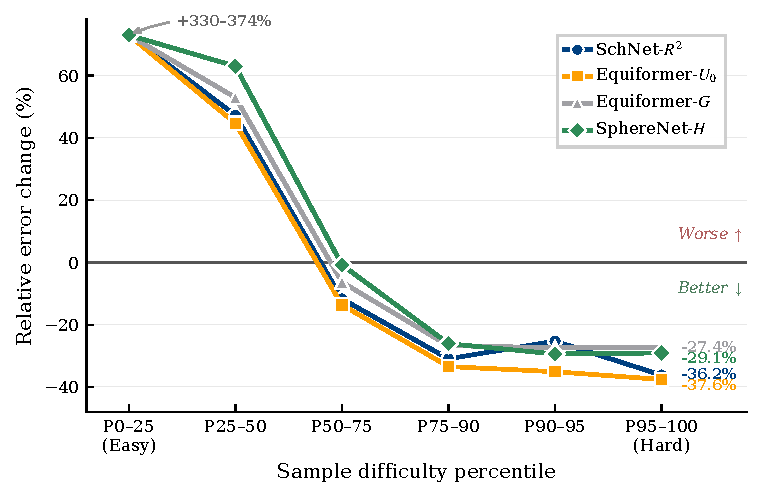
\includegraphics[width=0.55\textwidth]{imgs_edgpp/experiments/difficulty_stratification_lines.pdf}
\caption{Difficulty-stratified relative error change on QM9. All four tasks are plotted on a single panel; the y-axis shows the per-bin relative change in mean absolute error between the tuned-$\kappa$ and default-$\kappa$ configurations. Hard samples (P75--100) show consistent improvement of 25--38\%, while the crossover near P50--75 and the remarkably similar trajectories across architectures confirm that capacity reallocation is a general mechanism of adaptive thresholding. \textit{Note}: P0--25 values are truncated at the y-axis limit; actual relative degradation on easy samples ranges from +330\% to +374\%, but corresponds to negligible absolute error increases.}
\label{fig:difficulty_stratification}
\end{figure}

Figure~\ref{fig:difficulty_stratification} stratifies test samples into six difficulty percentiles and plots the relative per-bin error change for all four representative tasks. The picture is striking: every task traces a nearly identical monotonic descent from degradation on easy samples to improvement on hard samples, crossing zero near P50--75. In relative terms, easy samples (P0--25) suffer a large increase (+330--374\%), whereas hard samples (P95--100) achieve a 27--38\% reduction. Because the absolute errors of easy samples are near-zero under the default-threshold configuration, the large relative increase translates to a negligible absolute penalty; conversely, the moderate relative decrease on hard samples corresponds to a substantial absolute gain.

This difficulty-dependent behavior is the intended mechanism of threshold tuning: by raising $\kappa$ beyond the default, EDG++ applies stricter filtering that suppresses potentially misleading ED signals on samples where the default-threshold model already performs well, reallocating model capacity to under-optimized hard samples. The remarkable consistency of this crossover pattern across three architectures and four quantum properties provides strong evidence that capacity reallocation is a general mechanism of adaptive thresholding.

Robustness metrics further confirm variance reduction: standard deviation reductions of 5.3\% (SchNet-$R^2$), 16.6\% (Equiformer-$U_0$), 17.3\% (Equiformer-$G$), and 11.1\% (SphereNet-$H$). Maximum error reductions are pronounced for Equiformer: 39.1\% ($U_0$) and 37.9\% ($G$). For Equiformer-$U_0$, the maximum error decreases from 1.665 to 1.014, a 39\% reduction that substantially enhances reliability in practical applications.


\section{Property-Type Grouped Analysis}
\label{sec:appendix_property_group}

Table~\ref{tab:property_group} provides a detailed property-type grouped analysis of EDG++ improvements.

\begin{table}[!htb]
  \centering
  \caption{Property-type grouped analysis of EDG++ improvement over the no-distillation baseline on QM9. ``Avg $\Delta$'' denotes the mean relative improvement. ``Win'' denotes the number of properties improved.}
  \label{tab:property_group}
  \scriptsize
  \begin{tabular}{lcccccc}
    \toprule
    \multirow{2}{*}{Group} & \multicolumn{2}{c}{SchNet} & \multicolumn{2}{c}{Equiformer} & \multicolumn{2}{c}{SphereNet} \\
    \cmidrule(lr){2-3} \cmidrule(lr){4-5} \cmidrule(lr){6-7}
    & Avg $\Delta$ & Win & Avg $\Delta$ & Win & Avg $\Delta$ & Win \\
    \midrule
    Electronic & +2.24\% & 5/5 & +3.64\% & 4/5 & +1.96\% & 5/5 \\
    Thermo. & +3.70\% & 5/5 & +16.30\% & 5/5 & +5.52\% & 5/5 \\
    Vibrational & +2.30\% & 1/1 & $-$3.20\% & 0/1 & +4.40\% & 1/1 \\
    Structural & +6.40\% & 1/1 & +11.90\% & 1/1 & +1.90\% & 1/1 \\
    \midrule
    Overall & +3.20\% & 12/12 & +9.03\% & 10/12 & +3.64\% & 12/12 \\
    \bottomrule
  \end{tabular}
\end{table}


\section{Distillation Weight Sensitivity}
\label{sec:appendix_lambda}

Table~\ref{tab:lambda_sensitivity} reports the per-task $\lambda$ sensitivity under the default-threshold configuration.

\begin{table}[!htb]
  \scriptsize
  \centering
  \caption{$\lambda$ sensitivity (relative performance difference between best and worst $\lambda \in \{0.01, 0.5, 1.0\}$) under the default-threshold configuration ($\kappa_{batch}\!=\!\kappa_{all}\!=\!0$, $\beta\!=\!0$).}
  \label{tab:lambda_sensitivity}
    \begin{tabular}{lccc}
    \toprule
    \textbf{Task} & \textbf{SchNet} & \textbf{Equiformer} & \textbf{SphereNet} \\
    \midrule
    $\alpha$   & 1.19\% & 1.21\% & 3.52\% \\
    $C_v$      & 1.09\% & 1.34\% & 1.89\% \\
    $G$        & 2.37\% & 12.85\% & 4.59\% \\
    $\Delta\varepsilon$ & 0.71\% & 1.56\% & 1.74\% \\
    $H$        & 0.33\% & 5.62\% & 6.88\% \\
    $\varepsilon_{\text{HOMO}}$ & 1.79\% & 1.75\% & 0.92\% \\
    $\varepsilon_{\text{LUMO}}$ & 1.39\% & 1.62\% & 2.35\% \\
    $\mu$      & 1.20\% & 3.10\% & 1.94\% \\
    $R^2$      & 2.21\% & 15.26\% & 5.84\% \\
    $U_0$      & 1.94\% & 34.87\% & 7.34\% \\
    $U$        & 1.26\% & 11.06\% & 4.35\% \\
    ZPVE       & 2.21\% & 3.00\% & 0.96\% \\
    \midrule
    \textbf{Average} & \textbf{1.47\%} & \textbf{7.77\%} & \textbf{3.53\%} \\
    \bottomrule
    \end{tabular}
\end{table}


\section{Hyperparameter Configurations for EDG and EDG++}
\label{app:hyper}

We report the default configuration used for the main results in Tables~\ref{tab:rmd17_energy} and~\ref{tab:rmd17_force}, and the full search space in Appendix~\ref{sec:appendix_hyperparam}. On QM9, all three architectures share the same hyperparameter search. On rMD17, all experiments use global thresholding only ($\beta\!=\!0$), because rMD17 trains one model per molecule and every mini-batch is drawn from the conformation distribution of a single molecule; batch-local reliability statistics therefore converge to the global statistics in expectation, and per-batch variation becomes informative only in the multi-molecule QM9 setting (cf.\ Table~\ref{tab:ablation_beta}). An empirical validation of this choice on three representative rMD17 molecules is provided in Appendix~\ref{app:beta_rmd17}. SchNet and ViSNet on rMD17 use the out-of-the-box configuration ($\kappa_{all}\!=\!0$) to probe cross-architecture generality, whereas SphereNet additionally tunes $\kappa_{all}$ per molecule over $\{-1.5, -1, -0.5, 0, 0.5, 1.0, 1.5\}$ to characterize the upper bound of the approach. Per-molecule $\kappa_{all}$ tuning is restricted to SphereNet because the 50-sample rMD17 validation set limits the reliability of such tuning for additional architectures.


\section{Empirical Validation of $\beta\!=\!0$ on rMD17}
\label{app:beta_rmd17}

To validate our default choice of $\beta\!=\!0$ (global-only thresholding) for rMD17, we run a $\beta$ ablation on three representative molecules---Aspirin (large, complex), Salicylic acid (mid-size with hydroxyl groups), and Toluene (small, aromatic)---using SphereNet with $\kappa_{all}\!=\!0$ and $\lambda\!=\!0.001$. Each molecule is trained for 1{,}000 epochs at three values of $\beta\in\{0, 0.5, 1.0\}$. Table~\ref{tab:rmd17_beta_ablation} reports the test-set MAE.

\begin{table}[!htb]
  \scriptsize
  \centering
  \caption{rMD17 $\beta$ ablation on SphereNet ($\kappa_{all}\!=\!0$, $\lambda\!=\!0.001$, 1{,}000 epochs). On the average across three molecules, $\beta\!=\!0$ minimizes Energy MAE while Force MAE is essentially insensitive to $\beta$. On per-molecule basis, $\beta\!=\!0$ is best on Energy for 2/3 molecules with the largest gaps appearing on the more complex molecules (Aspirin and Salicylic). Bold indicates the best result per row.}
  \label{tab:rmd17_beta_ablation}
    \begin{tabular}{lccc}
    \toprule
    \textbf{Molecule} & $\beta\!=\!0$ & $\beta\!=\!0.5$ & $\beta\!=\!1.0$ \\
    \midrule
    \multicolumn{4}{l}{\textit{Energy MAE ($\frac{kcal}{mol}$)}} \\
    Aspirin       & \textbf{0.12406} & 0.18744 & 0.22103 \\
    Salicylic     & \textbf{0.06603} & 0.06894 & 0.09613 \\
    Toluene       & 0.02366 & 0.02252 & \textbf{0.02161} \\
    \emph{Average} & \textbf{0.07125} & 0.09297 & 0.11292 \\
    \midrule
    \multicolumn{4}{l}{\textit{Force MAE ($\frac{kcal}{mol\cdot \text{\r{A}}}$)}} \\
    Aspirin       & \textbf{0.38060} & 0.38130 & 0.38529 \\
    Salicylic     & 0.29756 & \textbf{0.29563} & 0.30040 \\
    Toluene       & 0.10518 & \textbf{0.10428} & 0.10462 \\
    \emph{Average} & 0.26111 & \textbf{0.26040} & 0.26344 \\
    \bottomrule
    \end{tabular}
\end{table}

The aggregate picture supports $\beta\!=\!0$ as the default for rMD17. On Energy MAE, $\beta\!=\!0$ achieves the lowest average error (0.07125 vs.\ 0.09297 for $\beta\!=\!0.5$ and 0.11292 for $\beta\!=\!1$); the gap is largest on the more complex molecules (Aspirin: 51\% lower than $\beta\!=\!0.5$; Salicylic: 4\% lower) and reverses only on Toluene with a small margin (9\% vs.\ $\beta\!=\!1$). On Force MAE, all three $\beta$ values perform within 1\% of each other (the average MAE differs by less than 0.003), reflecting that force prediction is dominated by local atomic interactions rather than the global energy distribution captured by ED. This empirical pattern matches the theoretical motivation in Appendix~\ref{app:hyper}: under per-molecule training, batch-local reliability statistics are noisy estimates of the same global distribution, and the small batch size in rMD17 (4 to 128 conformations of a single molecule) further amplifies noise; pure global thresholding ($\beta\!=\!0$) avoids this noise without losing distributional information.


\section{Progressive Component Ablation (SphereNet, rMD17)}
\label{app:progressive}

To isolate the contribution of the reliability estimator from that of the distillation weight and threshold tuning, we report a progressive-ablation study on SphereNet, the only rMD17 architecture for which the full configuration chain---EDG with tuned $\lambda$, EDG with fixed $\lambda\!=\!0.001$, EDG++ at $\kappa_{all}\!=\!0$, and EDG++ with tuned $\kappa_{all}$---is available. Table~\ref{tab:rmd17_progressive} reports MAE for each configuration.

\begin{table*}[!htb]
  \scriptsize
  \centering
  \caption{Progressive component ablation on SphereNet (rMD17). EDG with tuned $\lambda$ is the conference-version baseline; ``EDG ($\lambda\!=\!0.001$)'' is a controlled baseline sharing the $\lambda$ used by EDG++ but without the reliability estimator; ``EDG++ ($\kappa\!=\!0$)'' denotes the default-threshold EDG++ configuration; ``EDG++'' is the best $\kappa_{all}$ per molecule. Bold indicates the best result per column.}
  \label{tab:rmd17_progressive}
  \setlength{\tabcolsep}{4pt}
    \begin{tabular}{lcccccccccc}
    \toprule
    \textbf{Method} & Aspirin & Azobenz. & Benzene & Ethanol & Malona. & Naphth. & Paracet. & Salicylic & Toluene & Uracil \\
    \midrule
    \multicolumn{11}{l}{\textit{Energy MAE ($\frac{kcal}{mol}$)}} \\
    EDG (tuned $\lambda$) & 0.13622 & \textbf{0.06788} & 0.00413 & \textbf{0.03575} & \textbf{0.05659} & 0.02753 & 0.09934 & 0.09569 & 0.02413 & \textbf{0.03683} \\
    EDG ($\lambda\!=\!0.001$) & 0.18166 & 0.06603 & 0.00377 & 0.04695 & 0.05806 & 0.05216 & 0.10866 & 0.09713 & 0.03175 & 0.05925 \\
    EDG++ ($\kappa\!=\!0$) & 0.12584 & 0.07125 & \textbf{0.00341} & 0.04081 & 0.06767 & 0.02373 & 0.09734 & \textbf{0.06563} & 0.02367 & 0.05570 \\
    EDG++ & \textbf{0.12391} & 0.07125 & \textbf{0.00341} & \textbf{0.03575} & 0.06611 & \textbf{0.02256} & \textbf{0.09628} & \textbf{0.06563} & \textbf{0.02220} & 0.04841 \\
    \midrule
    \multicolumn{11}{l}{\textit{Force MAE ($\frac{kcal}{mol\cdot \text{\r{A}}}$)}} \\
    EDG (tuned $\lambda$) & 0.38598 & \textbf{0.21665} & 0.02101 & 0.18741 & \textbf{0.28456} & 0.11102 & 0.32023 & \textbf{0.28299} & 0.10804 & \textbf{0.17179} \\
    EDG ($\lambda\!=\!0.001$) & 0.38870 & 0.21670 & 0.02160 & \textbf{0.18594} & 0.29120 & 0.11220 & \textbf{0.31742} & 0.28919 & 0.10706 & 0.26561 \\
    EDG++ ($\kappa\!=\!0$) & 0.37960 & 0.22238 & 0.02078 & 0.18871 & 0.31599 & 0.09711 & 0.32309 & 0.29871 & \textbf{0.10341} & 0.23117 \\
    EDG++ & \textbf{0.37929} & 0.21708 & \textbf{0.02012} & 0.18698 & 0.31599 & \textbf{0.09541} & 0.31846 & 0.29452 & \textbf{0.10341} & 0.22544 \\
    \bottomrule
    \end{tabular}
\end{table*}

Comparing EDG ($\lambda\!=\!0.001$) to EDG++ ($\kappa\!=\!0$), which differ only in whether the reliability estimator is active, the estimator improves energy on 8/10 molecules, with naphthalene ($\downarrow$54.5\%), salicylic acid ($\downarrow$32.4\%), and aspirin ($\downarrow$30.7\%) showing the largest gains. Naive distillation at $\lambda\!=\!0.001$ without the estimator degrades energy below baseline on 4/10 molecules (e.g., naphthalene: $\uparrow$36.4\%); the estimator recovers 3 of these 4 cases to below-baseline error, indicating that reliability-aware filtering is essential for safe distillation at this weight. Threshold tuning (EDG++ $\kappa\!=\!0 \to$ EDG++ with tuned $\kappa$) provides further incremental gains.


\section{Boundary Case Analysis: Malonaldehyde}
\label{app:boundary}

Malonaldehyde is the only molecule where the reliability estimator consistently degrades performance on rMD17. Naive distillation at $\lambda\!=\!0.001$ improves energy (0.05806 vs.\ baseline 0.06005, $\downarrow$3.3\%), indicating that the ED-based distillation signal is beneficial for this molecule. Activating the estimator (EDG++ $\kappa\!=\!0$: 0.06767) reverses this gain, suggesting that the estimator incorrectly filters beneficial distillation signal, likely because the rapid intramolecular proton-transfer dynamics of malonaldehyde produce ED patterns that the estimator misclassifies as unreliable. EDG with per-task-best $\lambda$ achieves the best result (0.05659), and threshold tuning partially mitigates the degradation (EDG++ best $\kappa$: 0.06611 versus 0.06767 at $\kappa\!=\!0$), pointing to molecule-adaptive thresholding as a future direction. A per-sample error visualization for malonaldehyde together with two representative success cases (naphthalene, uracil) is given in Appendix~\ref{sec:appendix_rmd17_vis}.


\section{rMD17 Prediction Error Visualization}
\label{sec:appendix_rmd17_vis}

\begin{figure*}[!htb]
\centering
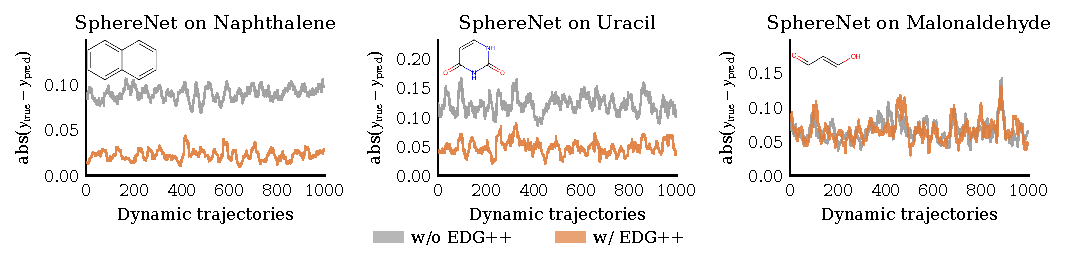
\includegraphics[width=\textwidth]{imgs_edgpp/experiments/rMD17_baseline_vs_edgpp.pdf}
\caption{Per-sample energy prediction errors on rMD17 (SphereNet), comparing the no-distillation baseline with EDG++ ($\kappa_{all}\!=\!1.5$ for naphthalene and uracil; $\kappa_{all}\!=\!1.0$ for malonaldehyde). We include three representative cases: two successes---naphthalene ($\Delta\!=\!+74.9\%$) and uracil ($\Delta\!=\!+60.4\%$)---and the identified boundary case, malonaldehyde ($\Delta\!=\!-0.2\%$), discussed in Appendix~\ref{app:boundary}, where the reliability estimator fails to filter beneficial distillation signal due to the molecule's rapid intramolecular proton-transfer dynamics. \textit{Note}: $\Delta$ values are computed from per-sample predictions of independently trained baseline and EDG++ models, not from the conference-version baselines in Tables~\ref{tab:rmd17_energy}--\ref{tab:rmd17_force}.}
\label{fig:rMD17_vis}
\end{figure*}


\section{Hyperparameter Interaction Analysis}
\label{sec:appendix_heatmap}

\begin{figure*}[!htb]
\centering

\includegraphics[width=\textwidth]{imgs_edgpp/experiments/heatmap_hyperparam.pdf}
\caption{Relative improvement (\%) over the no-distillation baseline as a function of $\kappa_{batch}$ and $\kappa_{all}$ with $\beta=0.5$ on QM9. For each ($\kappa_{batch}$, $\kappa_{all}$) pair, we report the best result across all $\lambda$ values. Blue indicates improvement; red indicates degradation; white corresponds to no change. Bold values denote $|\Delta|>5\%$. \textit{Note}: color scales are independently normalized per panel to maximize contrast within each task-model combination.}
\label{fig:heatmap_hyperparam}
\end{figure*}

Figure~\ref{fig:heatmap_hyperparam} visualizes the relative improvement over the baseline as a function of $\kappa_{batch}$ and $\kappa_{all}$ under the hybrid strategy ($\beta=0.5$) for four representative tasks. Two observations emerge. First, the improvement landscape is generally smooth, with most cells showing positive gains, indicating that EDG++ is robust to the specific choice of $\kappa$ values. Second, the optimal region varies by task and model: for SchNet, the improvements are uniformly distributed (all cells within 1\% of each other), while for SphereNet, thermodynamic properties like $G$ show more pronounced sensitivity to $\kappa_{all}$, with stricter filtering ($\kappa_{all}=1.5$) yielding larger gains.

\textbf{Threshold sensitivity on rMD17.} We further analyze how $\kappa_{all}$ affects energy prediction on rMD17 (SphereNet, $\lambda\!=\!0.001$). The sensitivity patterns are highly molecule-dependent: aspirin and toluene favor negative $\kappa_{all}$ (more inclusive filtering), while naphthalene and uracil favor positive $\kappa_{all}$ (stricter filtering). Malonaldehyde is the most extreme case, with energy improvement fluctuating between $-260\%$ and $+10\%$ across $\kappa_{all} \in [-1.5, 1.5]$, consistent with its challenging proton transfer dynamics. Force predictions are relatively insensitive to $\kappa_{all}$ across all molecules, suggesting that the ED teacher primarily provides global energy-level information rather than local force-level gradients.


\section{ImageED Reconstruction Visualization}
\label{sec:appendix_imageed_vis}

\begin{figure}[!htb]
\centering
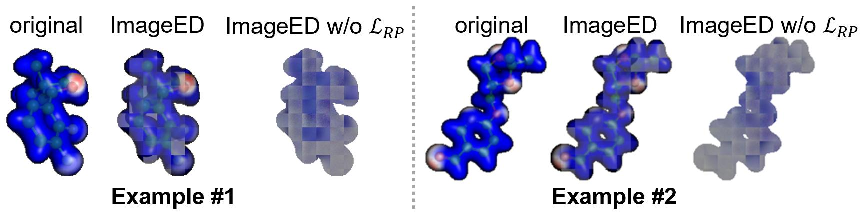
\includegraphics[width=\columnwidth]{imgs_edgpp/experiments/ImageED_output.pdf}
\caption{Visualization of ImageED reconstruction. ImageED generates high-quality ED images compared to the originals. Removing the masked reconstruction task ($\mathcal{L}_{MR}$) limits the understanding of local pixel-level features.}
\label{fig:vis_ImageED}
\end{figure}

Figure~\ref{fig:vis_ImageED} shows the reconstruction quality of ImageED. ImageED can faithfully reconstruct ED images compared to the originals, indicating that it effectively learns ED-related knowledge from the multi-view RGB-D images. Removing the masked reconstruction task (ImageED w/o $\mathcal{L}_{MR}$) degrades the reconstruction of local pixel-level details, confirming the importance of both pretext tasks.


\section{ED Image Representation Comparison}
\label{sec:appendix_ed_repr}

\begin{table}[!htb]
  \scriptsize
  \centering
  \caption{RMSE performance of different ED representations on 6 energy prediction tasks. Point cloud, voxel, and image use PointNet, ResNet3D, and ResNet18, respectively. E1--E6 represent DF-RKS Final Energy, Nuclear Repulsion Energy, One-Electron Energy, Two-Electron Energy, DFT Exchange-Correlation Energy, and Total Energy.}
  \label{tab:results_ED_images}
    \begin{tabular}{ccccccc}
    \toprule
    Repr. & E1 & E2 & E3 & E4 & E5 & E6 \\
    \midrule
    Point & 275.1 & 168.6 & 557.7 & 244.8 & 14.5 & 288.9 \\
    Voxel & 121.1 & 313.9 & 947.8 & 271.2 & 7.9 & 202.0 \\
    Image & \textbf{111.6} & \textbf{47.9} & \textbf{349.8} & \textbf{85.6} & \textbf{4.4} & \textbf{124.5} \\
    \midrule
    $\Delta$ & $\uparrow$7.8\% & $\uparrow$71.6\% & $\uparrow$37.3\% & $\uparrow$65.0\% & $\uparrow$44.5\% & $\uparrow$38.4\% \\
    \bottomrule
    \end{tabular}
\end{table}


\section{Computational Cost Analysis}
\label{sec:appendix_cost}

EDG++ introduces no additional parameters or forward passes beyond EDG; the only overhead is a scalar reliability score lookup per sample, resulting in $<$5\% per-epoch overhead compared to the no-distillation baseline. All experiments were conducted on 8$\times$ NVIDIA H200 GPUs. On QM9, a single distillation run takes $\sim$18h (SchNet, 1000 epochs), $\sim$35h (SphereNet, 1000 epochs), or $\sim$40h (Equiformer, 300 epochs). The dominant cost is the grid search: each model requires 45 configurations (3 $\lambda$ values $\times$ 15 $(\kappa, \beta)$ combinations) per task, totaling $\sim$9.6k, $\sim$19.0k, and $\sim$21.3k GPU-hours for SchNet, SphereNet, and Equiformer, respectively. On rMD17, SphereNet requires 7 $\kappa_{all}$ values per molecule ($\sim$46h per run), totaling $\sim$3.1k GPU-hours. In practice, the search can be substantially reduced by first identifying a good $\lambda$ on a representative task and then only searching over $(\kappa, \beta)$, which would reduce the search space by 3$\times$.


\section{Contribution Decomposition and Baseline Discussion}
\label{sec:appendix_contribution}

Our experimental design provides a natural two-level decomposition: Baseline $\to$ EDG isolates the contribution of ED as privileged information, and EDG $\to$ EDG++ isolates the contribution of reliability-aware selective distillation.

\textbf{Why standard KD baselines are not included.} We acknowledge that comparisons with adapted standard KD baselines (\eg, FitNets~\cite{romero2015fitnets}, AT~\cite{zagoruyko2017paying}) would strengthen the paper. In principle, one could implement a ``structural-image teacher $\to$ geometry student'' feature matching control without ED pre-training, which would help disentangle whether the gains come from (1)~the ED signal itself, (2)~the auxiliary teacher architecture, or (3)~the cross-modal training paradigm. We did not include such controls due to computational budget constraints: the full EDG++ grid search already required $\sim$50k GPU-hours.

However, several lines of indirect evidence support that the gains primarily originate from the ED signal rather than the teacher architecture \emph{per se}: (i)~the improvement hierarchy across property types (thermodynamic $>$ electronic $>$ vibrational) is physically consistent with the Hohenberg-Kohn theorem---a generic teacher architecture would not produce this pattern; (ii)~the improvements are consistent across four fundamentally different student architectures (SchNet, Equiformer, SphereNet, ViSNet), suggesting the transferred knowledge is architecture-agnostic; (iii)~the reliability estimator, trained to predict \emph{ED reconstruction error}, is effective at identifying samples where distillation helps---this would not work if the gains were unrelated to ED quality. We encourage future work to include a non-ED teacher control to formally validate this decomposition.


\section{Dataset Descriptions}
\label{sec:appendix_datasets}

\subsection{QM9 Dataset}

QM9~\cite{ramakrishnan2014quantum} is a widely used benchmark for quantum chemistry, containing 133,885 small organic molecules with up to 9 heavy atoms (C, N, O, F). Each molecule is associated with 12 quantum mechanical properties computed using density functional theory (DFT) at the B3LYP/6-31G(2df,p) level. Table~\ref{tab:qm9_properties} provides detailed descriptions of these properties.

\begin{table}[!htb]
  \centering
  \caption{Descriptions of 12 quantum mechanical properties in QM9.}
  \label{tab:qm9_properties}
  \scriptsize
    \begin{tabular}{clcc}
    \toprule
    \textbf{Property} & \textbf{Description} & \textbf{Unit} & \textbf{Type} \\
    \midrule
    $\alpha$ & Isotropic polarizability & $a_0^3$ & Electronic \\
    $\Delta\varepsilon$ & HOMO-LUMO gap & meV & Electronic \\
    $\varepsilon_{HOMO}$ & Highest occupied molecular orbital energy & meV & Electronic \\
    $\varepsilon_{LUMO}$ & Lowest unoccupied molecular orbital energy & meV & Electronic \\
    $\mu$ & Dipole moment & D & Electronic \\
    $C_v$ & Heat capacity at 298.15K & $\frac{cal}{mol \cdot K}$ & Thermodynamic \\
    $G$ & Free energy at 298.15K & meV & Thermodynamic \\
    $H$ & Enthalpy at 298.15K & meV & Thermodynamic \\
    $R^2$ & Electronic spatial extent & $a_0^2$ & Structural \\
    $U$ & Internal energy at 298.15K & meV & Thermodynamic \\
    $U_0$ & Internal energy at 0K & meV & Thermodynamic \\
    ZPVE & Zero point vibrational energy & meV & Vibrational \\
    \bottomrule
    \end{tabular}
\end{table}

\subsection{rMD17 Dataset}

The revised MD17 (rMD17)~\cite{christensen2020role} dataset contains molecular dynamics trajectories for 10 small organic molecules. Each trajectory consists of molecular conformations with corresponding energies and atomic forces computed at the PBE+vdW-TS level of theory. Table~\ref{tab:rmd17_molecules} provides detailed descriptions of these molecules.

\begin{table}[!htb]
  \centering
  \caption{Descriptions of 10 molecules in rMD17.}
  \label{tab:rmd17_molecules}
  \scriptsize
    \begin{tabular}{clccc}
    \toprule
    \textbf{No.} & \textbf{Molecule} & \textbf{Formula} & \textbf{\#Atoms} & \textbf{\#Conformations} \\
    \midrule
    1 & Aspirin & C$_9$H$_8$O$_4$ & 21 & 211,762 \\
    2 & Azobenzene & C$_{12}$H$_{10}$N$_2$ & 24 & 99,999 \\
    3 & Benzene & C$_6$H$_6$ & 12 & 627,983 \\
    4 & Ethanol & C$_2$H$_6$O & 9 & 555,092 \\
    5 & Malonaldehyde & C$_3$H$_4$O$_2$ & 9 & 993,237 \\
    6 & Naphthalene & C$_{10}$H$_8$ & 18 & 326,250 \\
    7 & Paracetamol & C$_8$H$_9$NO$_2$ & 20 & 106,490 \\
    8 & Salicylic acid & C$_7$H$_6$O$_3$ & 16 & 320,231 \\
    9 & Toluene & C$_7$H$_8$ & 15 & 442,790 \\
    10 & Uracil & C$_4$H$_4$N$_2$O$_2$ & 12 & 133,770 \\
    \bottomrule
    \end{tabular}
\end{table}


\section{Paired Bootstrap Confidence Intervals}
\label{sec:appendix_bootstrap}

To quantify the estimation uncertainty of our single-seed results, we compute paired bootstrap 95\% confidence intervals based on per-sample test predictions (10,831 samples for QM9). For each task-model pair, we resample the test set 10,000 times with replacement and compute the MAE on each resample. Table~\ref{tab:bootstrap_ci} reports the bootstrap CI for representative tasks.

\begin{table}[!htb]
  \centering
  \caption{Bootstrap 95\% CIs for EDG++ (per-task-best) and paired bootstrap test of EDG++ vs.\ EDG on representative QM9 tasks. $\Delta$: paired difference in MAE (EDG $-$ EDG++; positive means EDG++ is better).}
  \label{tab:bootstrap_ci}
  \scriptsize
  \begin{tabular}{llccc}
    \toprule
    \textbf{Model} & \textbf{Task} & \textbf{EDG++ MAE [95\% CI]} & \textbf{$\Delta$ [95\% CI]} & \textbf{$p$} \\
    \midrule
    SchNet & $R^2$ & 0.126 [0.121, 0.132] & +0.003 [+0.000, +0.006] & 0.020 \\
    Equif. & $U_0$ & 0.017 [0.016, 0.018] & +0.001 [+0.001, +0.002] & $<$0.001 \\
    Equif. & $\mu$ & 0.021 [0.020, 0.022] & 0.000 & n.s. \\
    Sphere. & $H$ & 0.006 [0.006, 0.007] & +0.000 [$-$0.000, +0.000] & 0.472 \\
    Sphere. & ZPVE & 0.001 [0.001, 0.001] & +0.000 [+0.000, +0.000] & 0.003 \\
    \bottomrule
  \end{tabular}
\end{table}

The mean relative CI width across all 36 task-model pairs is 7.0\% (median 6.1\%, max 12.5\%), indicating that the single-seed point estimates are reasonably stable. The paired bootstrap tests confirm that several key improvements (Equiformer-$U_0$, SphereNet-ZPVE) are statistically robust even within a single seed ($p < 0.01$), while others (SphereNet-$H$) require multi-seed evaluation for definitive conclusions.


\section{Hyperparameter Search Space}
\label{sec:appendix_hyperparam}

We conduct grid search over the following hyperparameters for EDG++:

\begin{itemize}
    \item \textbf{Distillation weight} $\lambda \in \{0.01, 0.5, 1.0\}$ for QM9; $\lambda = 0.001$ for rMD17
    \item \textbf{Local threshold coefficient} $\kappa_{batch} \in \{-1.5, 0, 1.5\}$
    \item \textbf{Global threshold coefficient} $\kappa_{all} \in \{-1.5, 0, 1.5\}$ for QM9; $\{-1.5, -1, -0.5, 0, 0.5, 1.0, 1.5\}$ for rMD17
    \item \textbf{Mixing coefficient} $\beta \in \{0, 0.5, 1.0\}$ for QM9; $\beta = 0$ for rMD17
\end{itemize}

For each task, we select the hyperparameter configuration that achieves the best validation performance.


\section{Implementation Details}
\label{sec:appendix_implementation}

\subsection{ImageED Pre-training}

The encoder and decoder of ImageED are built based on ViT-Base/16~\cite{dosovitskiy2020image}. The encoder has an embedding dimension of 768 with 12 Transformer layers, and the decoder has an embedding dimension of 512 with 8 Transformer layers. We use a learning rate of 1.5e-4, a batch size of 64, a mask ratio of 0.25, $\lambda_{VR}=1$ and $\lambda_{MR}=1$ for 20 epochs on 8 GeForce RTX 4090 GPUs. The input ED images have shape $6 \times 4 \times 224 \times 224$ (6 views, 4 channels including RGB-D).

\subsection{ED-aware Teacher Pre-training}

We divide 2\% of the 2 million molecules as validation set and the rest as training set. The ED-aware teacher uses ResNet18~\cite{he2016deep} with view-wise average pooling. The ED predictor is a 2-layer MLP with Softplus activation. We use a learning rate of 5e-3 and a batch size of 128 to train for approximately 280k steps.

\subsection{Reliability Estimator Training}

The reliability estimator is a lightweight MLP with architecture: Linear(512, 256) $\rightarrow$ Softplus $\rightarrow$ Linear(256, 1), with approximately 131K parameters. It is jointly trained with the ED-aware teacher and ED predictor in Stage II, sharing the same SGD optimizer (momentum 0.9, learning rate 0.003, weight decay 1e-4, batch size 128, 25 epochs). Note that the evaluator's input features are detached from the teacher's computation graph to prevent gradient interference. The training objective is to predict the L2 reconstruction error between predicted and ground-truth ED features.

\subsection{Downstream Task Training}

For QM9, we use the dataset split from Geom3D~\cite{liu2024symmetry}: 110K for training, 10K for validation, and 11K for testing. For rMD17, we use 950 for training, 50 for validation, and 1000 for testing. The mapper $f_M$ and task predictor $f_T$ each consist of a single linear layer. We select the best checkpoint based on validation MAE for QM9 and validation force MAE for rMD17.


\vfill

\end{document}
